\chapter{Autoregulon Networks: COMING SOON}
\label{ch-autoregulons}

This chapter is heavily based on Ref.\cite{alon-book},
which I highly recommend. That book divides its chapters into 3 \qt{Parts}: Network Motifs, Robustness and Optimality. This chapter covers only the first part, Network Motifs (NM). Autoregulon networks
is an alternative name for NM. 

This chapter only covers the 
causal aspects of NM. It does no justice to the cell biology and organic chemistry underpinning NM. For that, please go to  Ref.\cite{alon-book}. 
This chapter will discuss a  special 
class of 
S1ODE (system of first order ordinary differential equations)
from a causal inference perspective. Ref.\cite{alon-book} describes the math 
behind such S1ODEs and also the place where they occur in Nature and even experimental data which supports that they are 
physically realized. The scope of this chapter is much more limited. We mostly confine ourselves
to discussing only the math behind such S1ODEs.
We do occasionally describe briefly some of the  genomics underpinings of the math.
If you are new to genomics, and would like to follow that discussion, you might find Appendix \ref{ch-genomics-vocab} helpful.


\section{Hill functions}

Two kinds of Hill functions.

Highpass filter ({
\bf activator}) Hill function
 \beqa
 f_{hp}(x) &=&\beta\frac{\left(\frac{x}{K}\right)^n}{1 + \left(\frac{x}{K}\right)^n}
 \\
 &\rarrow& \beta\indi(x>K) \text{ as } n\rarrow\infty
 \eeqa
 
 Lowpass filter ({\bf repressor}) Hill fuction
 \beqa
  f_{lp}(x) &=&\beta\frac{1}{1 + \left(\frac{x}{K}\right)^n}
  \\
  &\rarrow& \beta\indi(x<K) \text{ as } n\rarrow\infty
  \eeqa


\begin{figure}[h!]
\centering
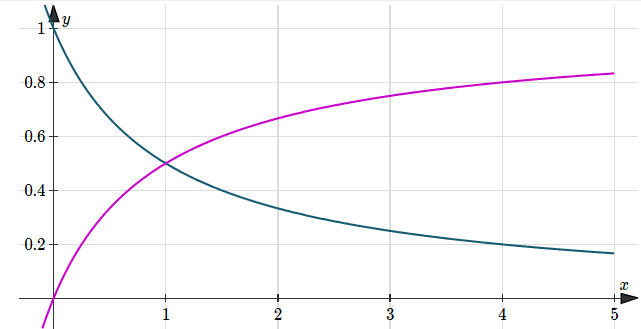
\includegraphics[width=4.3in]
{autoregulons/hill-1.png}
\caption{Plot of $y= 1/(1+x^n)$
and $y=x^n/(1+x^n)$ for $n=1$.}
\label{fig-hill-1.png}
\end{figure}

\begin{figure}[h!]
\centering
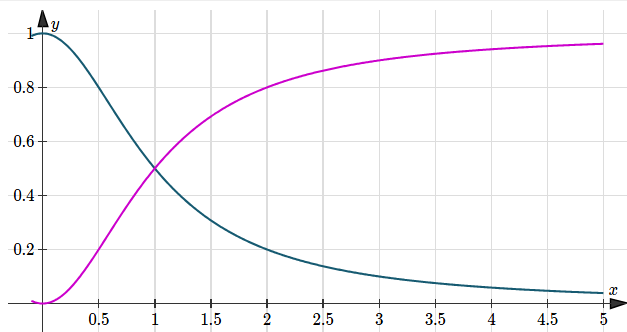
\includegraphics[width=4.3in]
{autoregulons/hill-2.png}
\caption{Plot of $y= 1/(1+x^n)$
and $y=x^n/(1+x^n)$ for $n=2$.}
\label{fig-hill-2.png}
\end{figure}

\begin{figure}[h!]
\centering
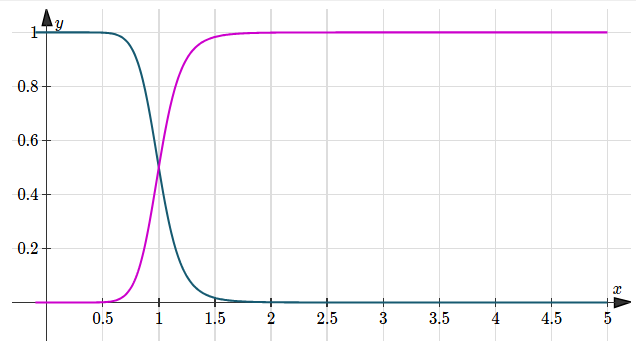
\includegraphics[width=4.3in]
{autoregulons/hill-10.png}
\caption{Plot of $y= 1/(1+x^n)$
and $y=x^n/(1+x^n)$ for $n=10$.}
\label{fig-hill-10.png}
\end{figure}

\section{One Autoregulon}
a {\bf net motif} is just a subgraph of a bnet

\begin{figure}[h!]
$$
\xymatrix{
&\rvx\ar[dd]|{-\alp}\ar[dl]
\\
f(\rvx)\ar[dr]|{1}
\\
&\Circle{\frac{d\rvx}{dt}}
}\quad
\xymatrix{\\=}
\quad
\xymatrix{
\\
\rvx\ar@{=>}[d]
\\
\dot{\rvx}
}
\xymatrix{\\=}
\quad
\xymatrix{\\\Rect{\rvx}}
$$
\caption{Autoregulon net motif and the 2 symbols that we will
use to denote it when we consider
networks of connected autoregulons. Assume $\alp >0$.}
\label{fig-net-motif}
\end{figure}

\beq
\frac{dx}{dt}=-\alp x + f(x)
\eeq
Let $\alp, \beta >0$.
In general, $f(x)$ is either the $hp$ or $lp$ Hill function.
However, we often use the following approximations
\beq
f(x)=\left\{
\begin{array}{ll}
\beta\indi(x>K)
&(\text{highpass filter})
\\
\beta\indi(x<K)
&(\text{lowpass filter})
\\
|f_1| x
&(\text{positive feedback})
\\
-|f_1| x
&(\text{negative feedback})
\end{array}
\right.
\eeq

\subsection{Linear Expansion of $f$}

Let 

\beq
\dot{x} = -\alp x + f(x) \quad\text{ with }
f(x)\approx f_0 + f_1x
\eeq
If
\beq
x_0 = x(0)\;,\;\;
\alp_1=\alp-f_1
\eeq
then the most general solution for $x(t)$ is
\beq
x(t)=\underbrace{x_0 e^{-\alp_1 t} }_{x_h}+
\underbrace{\frac{f_0}{\alp_1}\left[1-e^{-\alp_1 t}\right]}_{x_p}
\eeq
as can be easily checked.
$x_h$ is called the {\bf homogeneous solution}\footnote{
$x_h$ satisfies the homogeneous ODE, i.e., the
ODE with $f(x)=0$.
}
and $x_p$ is called the {\bf particular solution}.
\footnote{
If we integrate both sides of
$\frac{dx}{f_0 -\alp_1 x}=dt$,
we only get the particular solution.}
Hence 
\begin{itemize}
\item
if $\alp-f_1=\alp_1<0$, then $x(t)$ 
goes exponentially fast  from $x_0$ to $(x_0 -\frac{f_0}{\alp_1})e^{|\alp_1|t}$
as $t\rarrow \infty$. 
\item 
if $\alp-f_1=\alp_1>0$, then $x(t)$ goes exponentially fast from
$x_0$ to $\frac{f_0}{\alp_1}$ as $t\rarrow \infty$.

\item if $f_1>0$ (positive feedback), then if it is strong
enough (i.e., if $f_1 > \alp$), then $\alp_1<0$ 
\item if $f_1<0$ (negative feedback), then $\alp_1>0$.
\end{itemize}

\subsection{Lowpass $f$}
If $f$ is a lowpass filter
\beq
x= 
\left\{
\begin{array}{ll}
x_0 e^{-\alp t} +
\frac{\beta}{\alp}\left[1-e^{-\alp t}\right]
&\text{ if } t<t_K
\\
x_K e^{-\alp (t-t_K)}
&\text{ if } t>t_K
\end{array}
\right.
\eeq
where, to make $x(t)$ continuous at $t=t_K$ and $x(t_K)=x_K$,
we must have

\beq
 x_0 e^{-\alp t_K} +
\frac{\beta}{\alp}
\left[1-e^{-\alp t_K}\right]
=
x_K
\eeq

Note that if $\alp t<<1$, then\footnote{Use $e^x\approx 1 + x$ for $|x|<<1$.}, 

\beqa
x &\approx&
x_0(1-\alp t) +\beta t
\\ &=&
x_0 + (\beta -\alp x_0)t
\eeqa

Assume $x_0=0$ for simplicity.
In that case, if $K>\frac{\beta} {\alp}$, $t_K$ 
doesn't exist and only the $t<t_K$
branch of the $x$ solution above exists.
On the other hand, if $K<\frac{\beta} {\alp}$, 
then $t_K$ exists and $x_K=K$.
For $t>t_K$,

\beq
x=
K e^{-\alp(t-t_K)}
\eeq

\begin{figure}[h!]
\centering
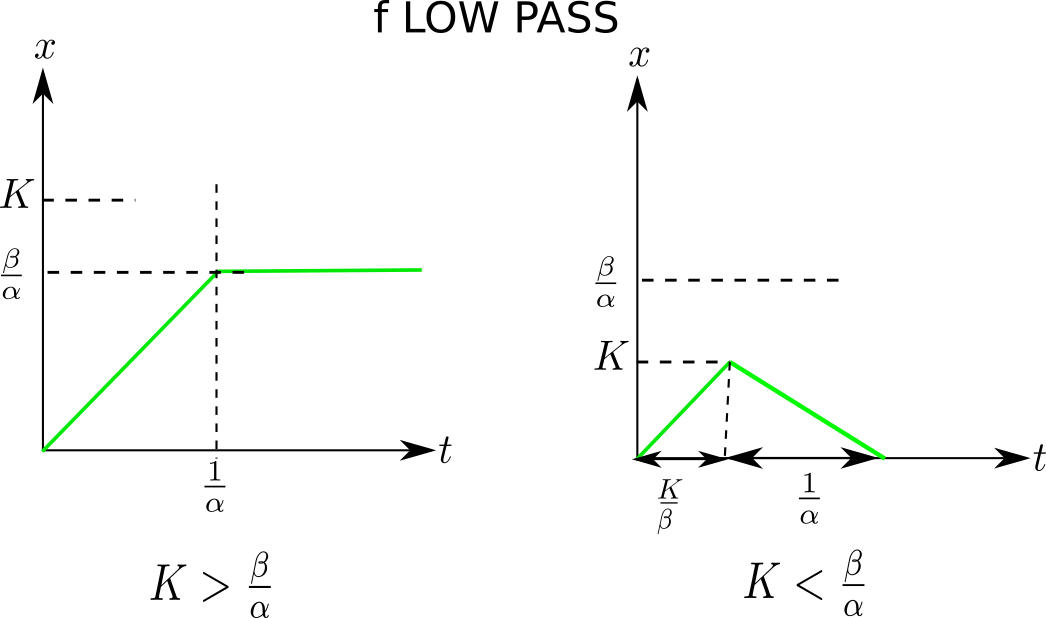
\includegraphics[width=4in]
{autoregulons/autoreg-lowpass.png}
\caption{Approximate $x$ for autoregulon with lowpass $f$
and $x_0=0$}
\label{fig-autoreg-lowpass}
\end{figure}

See Fig.\ref{fig-autoreg-lowpass}
for approximate 
$x$ for autoregulon with lowpass $f$
and $x_0=0$.

Autoregulon with lowpass $f$ can be used for {\bf memory}.


\subsection{Highpass $f$}
For $f$ is a highpass filter

\beq
x= 
\left\{
\begin{array}{ll}
x_0 e^{-\alp t} &\text{ if } t<t_K  
\\
x_K e^{-\alp (t-t_K)} +
\frac{\beta}{\alp}
\left[ 1-e^{-\alp (t-t_K)}\right]
&\text{ if } t>t_K
\end{array}
\right.
\eeq
where, to make $x(t)$ continuous at $t=t_K$ and $x(t_K)=x_K$,
we must have

\beq
x_0 e^{-\alp t_K} = x_K
\eeq

Note that if $\alp t<<1$, then

\beqa
x &\approx&
x_0(1 -\alp t)
\eeqa
Unlike when $f$ is lowpass, 
in this case of $f$ highpass,
we can't assume $x_0=0$ or else $x_K=K=0$ too. In fact, we must have $x_0 > x_K=K$. For $\alp (t-t_K) >>1$, 
\beq
x\approx \frac{\beta}{\alp}
\eeq

\begin{figure}[h!]
\centering
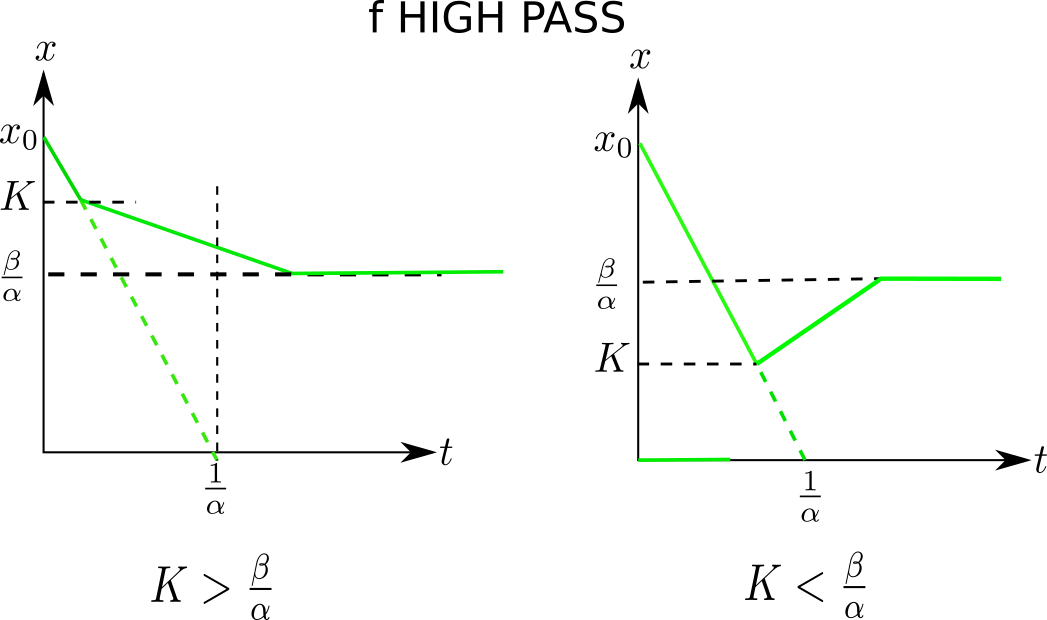
\includegraphics[width=4in]
{autoregulons/autoreg-highpass.png}
\caption{Approximate $x$ for autoregulon with highpass $f$}
\label{fig-autoreg-highpass}
\end{figure}
See Fig.\ref{fig-autoreg-highpass}
for picture of 
approximate $x$ for autoregulon with highpass $f$.




\subsection{Acceleration towards attracting point}

Assume 

\beq
f(x)\approx f_0^a + f_1^a (x-x_a)
\eeq

\begin{figure}[h!]
\centering
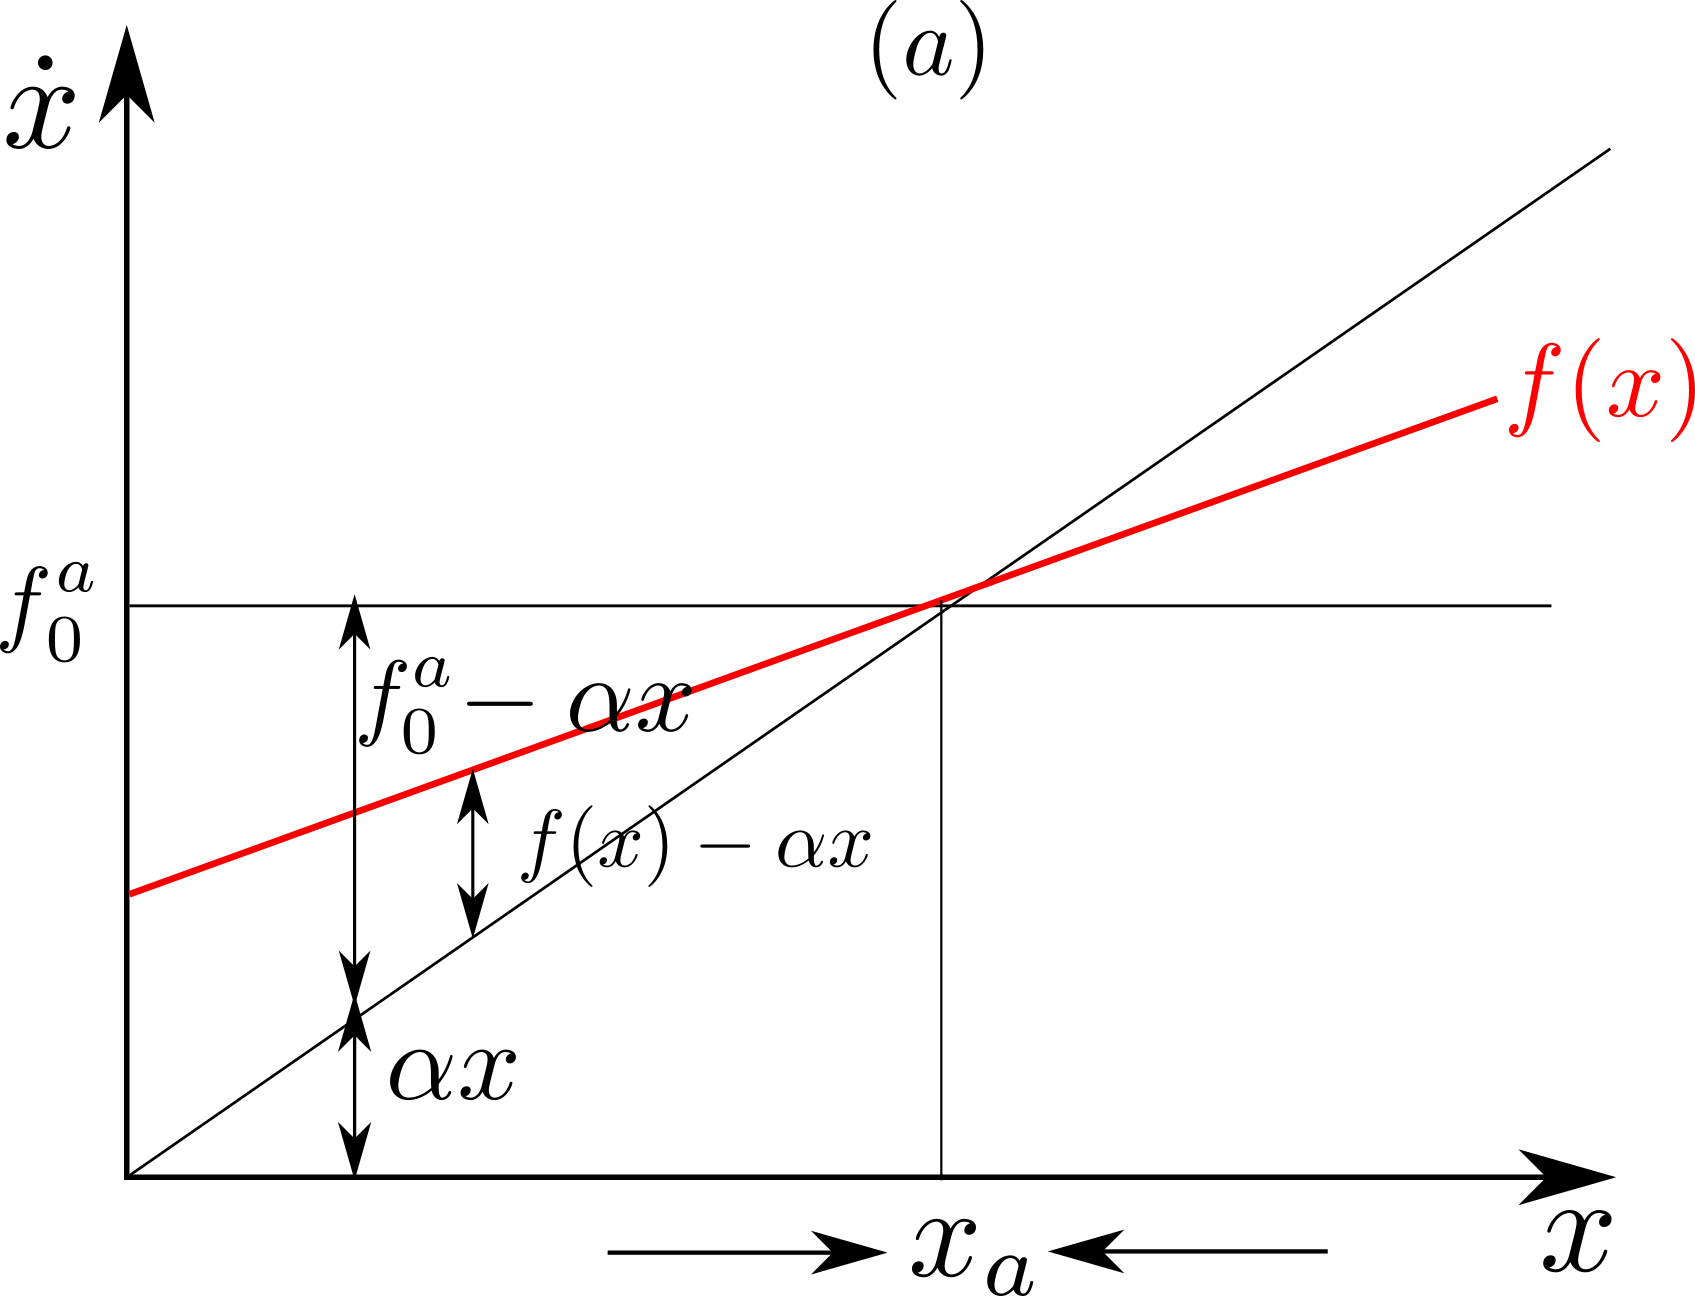
\includegraphics[width=2.5in]
{autoregulons/xdot-versus-x.png}
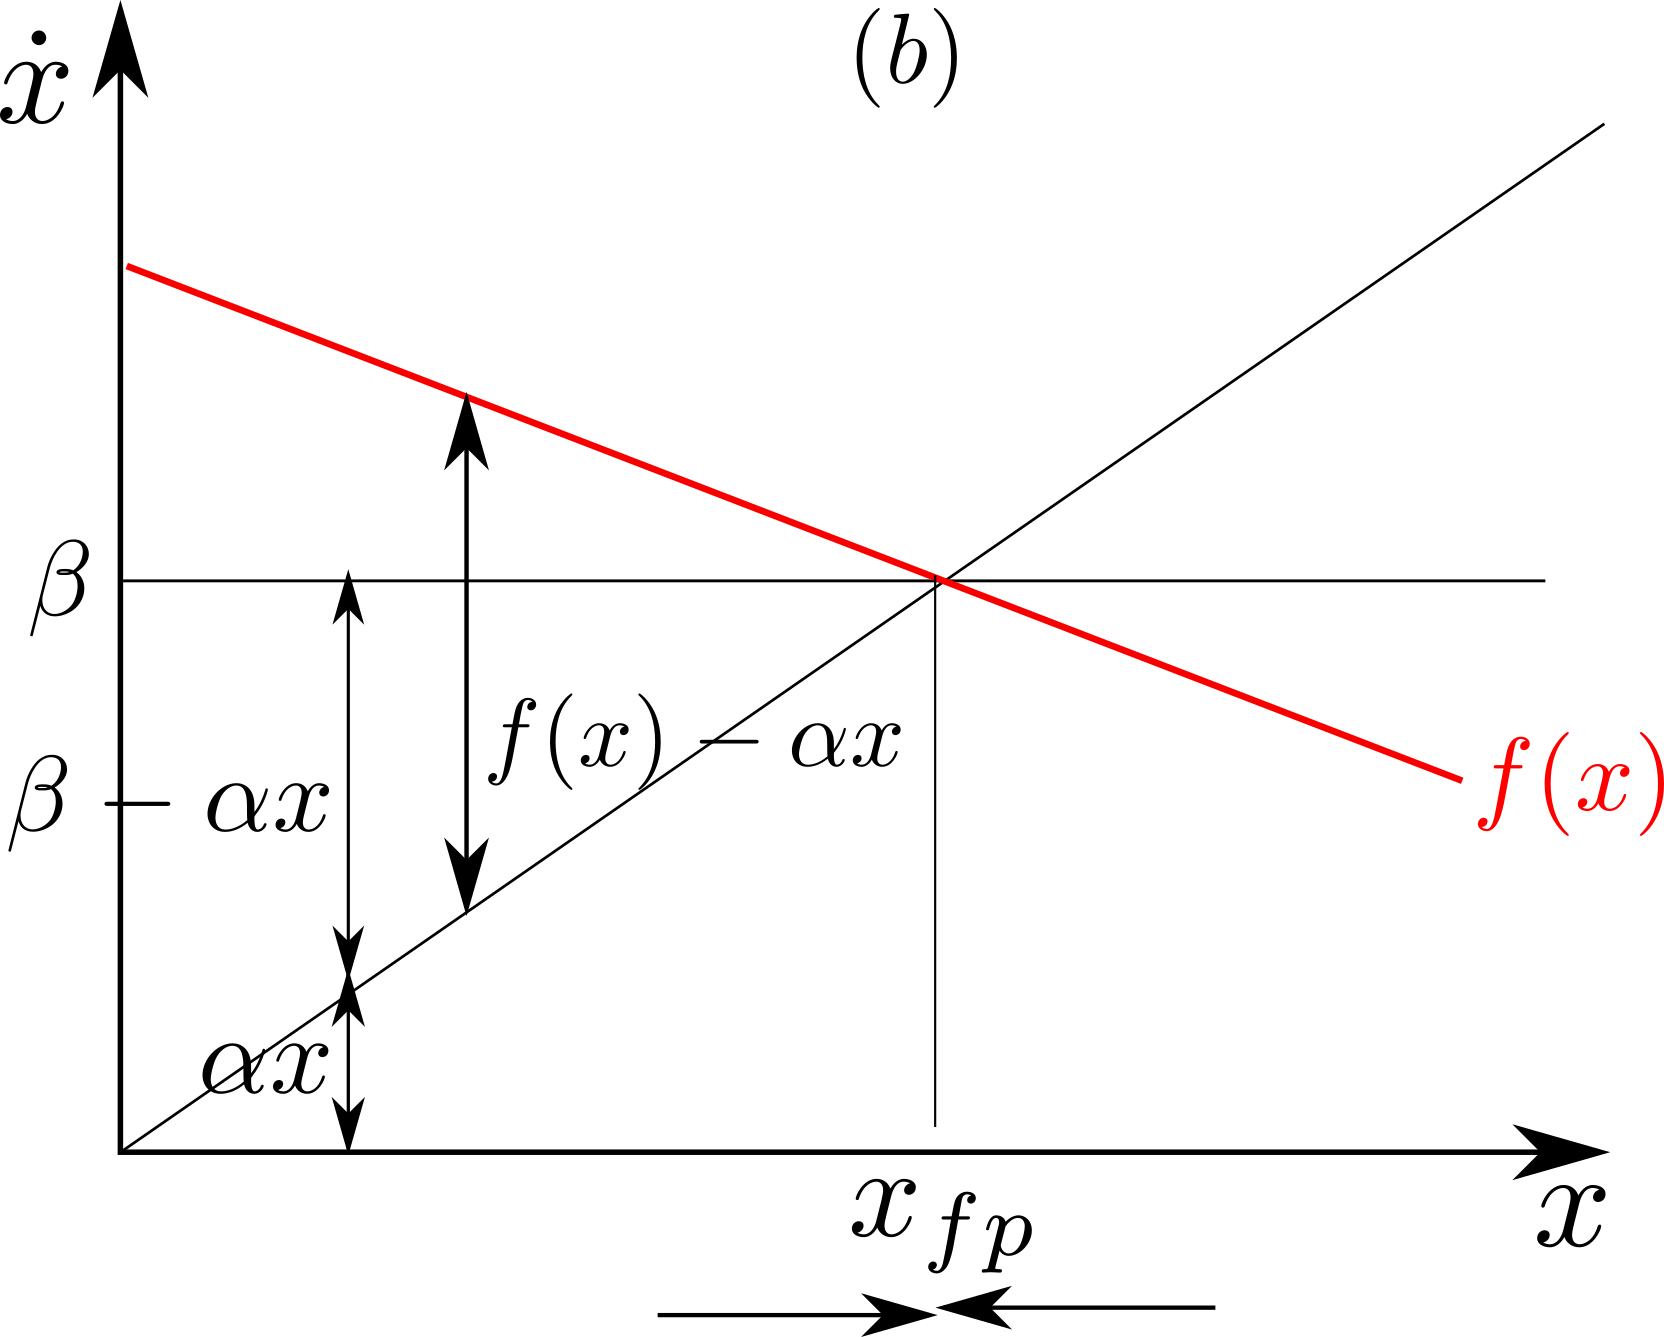
\includegraphics[width=2.5in]
{autoregulons/xdot-versus-x-neg.png}
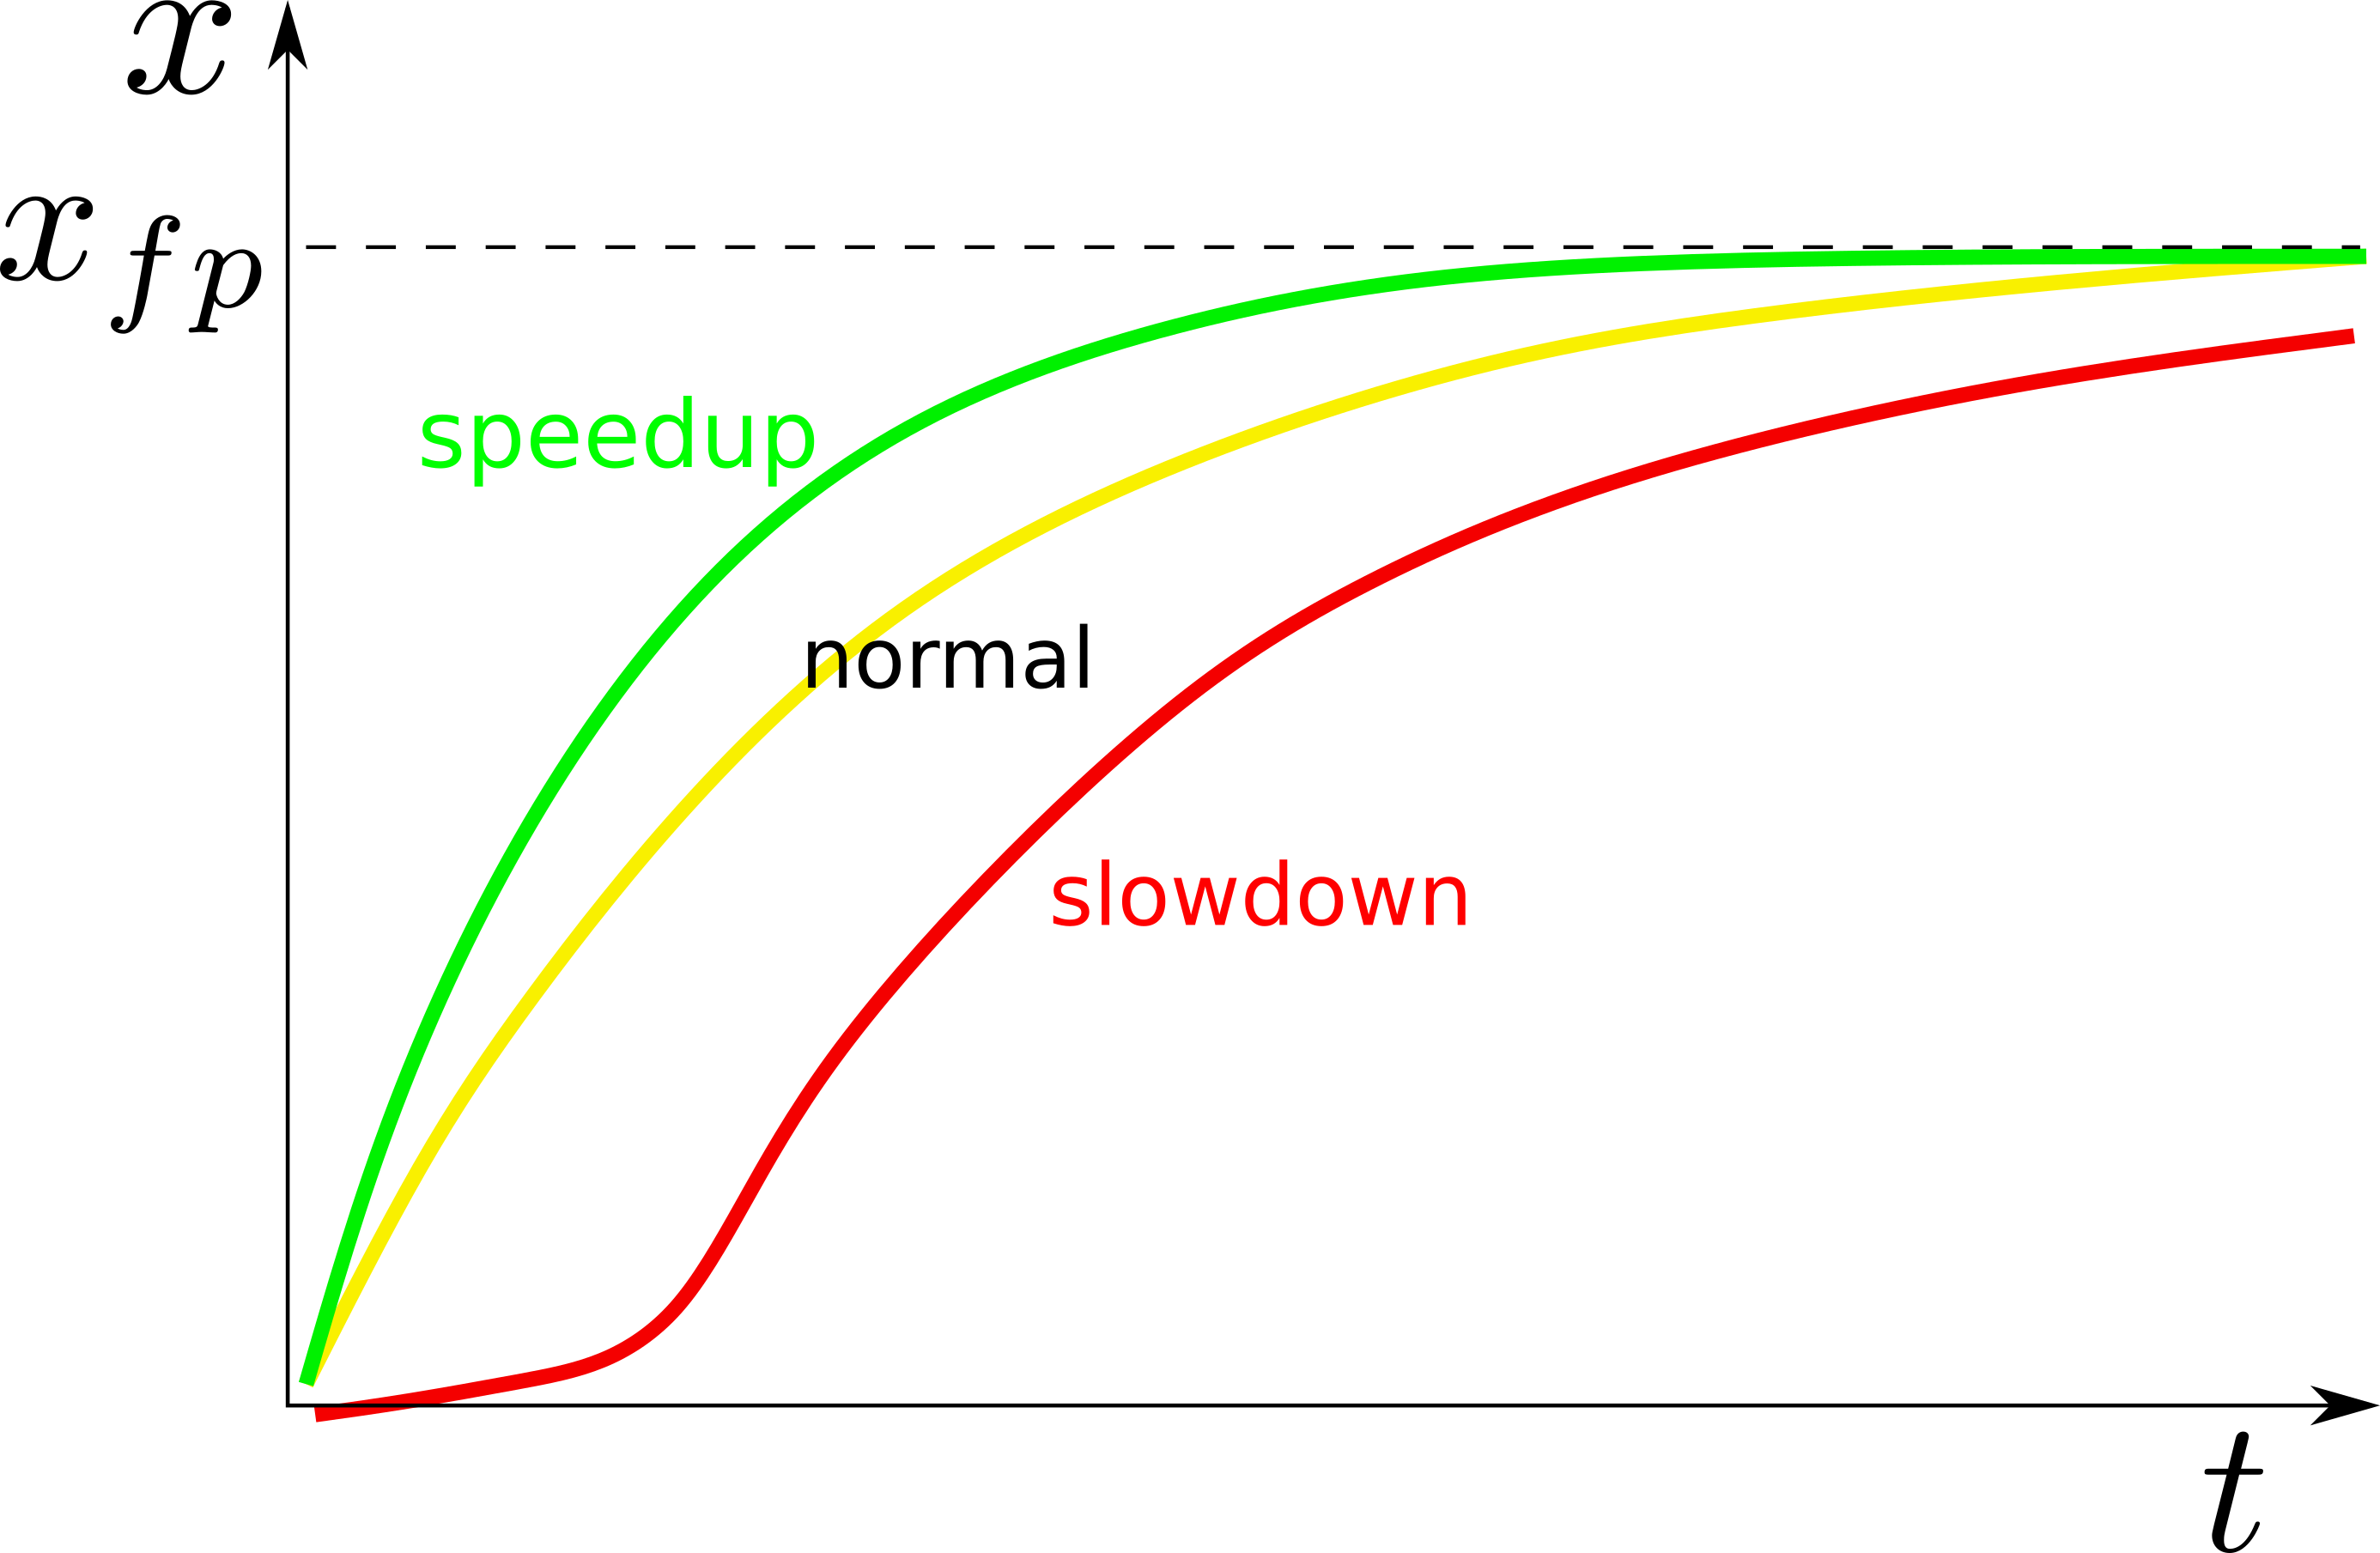
\includegraphics[width=2.5in]
{autoregulons/fast-normal-slow.png}
\caption{For single autoregulon, $\dot{x}(t)=-\alp x + f(x)$ with $f(x)=f_0^a + f^a_1(x-x_a)$.
Slowdown ($f_1^a>0$),
Speedup ($f_1^a<0$),  Normal ($f_1^a=0$)
 }
\label{fig-fast-normal-slow}
\end{figure}

Define
\begin{itemize}
\item
{\bf positive autoregulation (PAR)}: $f_1^a >0$, positive slope at $x=x_a$, , slowdown
\item
{\bf negative autoregulation (NAR)}: $f_1^a <0$, negative slope at $x=x_a$, speedup
\item
{\bf zero autoregulation (ZAR)}: $f_1^a =0$, zero slope at $x=x_a$,\qt{normal} speed
\end{itemize}
These definitions are illustrated in Fig.\ref{fig-fast-normal-slow}.

\section{Autoregulon notation}
Henceforth, we will use

\begin{itemize}
\item
$\xymatrix{\Rect{\rvx}}$ to denote any 
autoregulon $\rvx$

\item
$\xymatrix{\Rect{\rvx^\redoplus}}$ to denote a highpass 
autoregulon $\rvx$

\item
$\xymatrix{\Rect{\rvx^\redominus}}$ to denote a lowpass 
autoregulon $\rvx$

\item
$\xymatrix{\Rect{\rvx^\redplus}}$ to denote a positive feedback 
autoregulon $\rvx$


\item  $\xymatrix{\Rect{\rvx^\redminus}}$
to denote a negative feedback 
autoregulon $\rvx$. \footnote{
Ref.\cite{alon-book}
denotes a negative feedback autoregulon by 
$\xymatrix{\rvx\loopright{3}{@{-|}}}$
} 

\item $\xymatrix{\rvx\ar[r]^\alp&\rvy}$ if $\rvy = \alp \rvx$.

 \item  $\xymatrix{\rvx\ar[r]|\redplus&\rvy}$
to denote
$\xymatrix{\rvx\ar[r]^\alp&\rvy}
$
with $\alp>0$.

\item  $\xymatrix{\rvx\ar[r]|\redminus&\rvy}$
to denote
$\xymatrix{\rvx\ar[r]^\alp&\rvy}$
with $\alp<0$\footnote{
Ref.\cite{alon-book}
represents $\xymatrix{\rvx\ar[r]|\redminus&\rvy}$ as $\xymatrix{\rvx\ar@{-|}[r]&\rvy}$
}

\item  $\xymatrix{\rvx\ar[r]|\redzero&\rvy}$
to denote
$\xymatrix{\rvx\ar[r]^\alp&\rvy}$
with $\alp=0$.

\item  $\xymatrix{\rvx\ar[r]|\redominus^K
&\rvy}$
to denote
$\rvy = \indi(\rvx< K)$
(i.e., lowpass filter)
for some $K>0$

\item  $\xymatrix{\rvx\ar[r]|\redoplus^K
&\rvy}$
to denote
$\rvy = \indi(\rvx> K)$
(i.e., highpass filter)
for some $K>0$.

\end{itemize}

Note that a highpass filter,
when smooth out 
to behave as its realization in Nature, has a steep section with positive slope, so a highpass filter
is closely related to positive feedback, as their symbols
$\redoplus$ and $\redplus$ suggest. Think of $\redoplus$ as an extreme sort of $\redplus$.

The last paragraph is still true if we replace (highpass,$\redoplus$, 
$\redplus$) by 
(lowpass,$\redominus$, 
$\redminus$).

If an arrow in a net has no sign, assume its sign is positive.



\section{Fixed Points}

\begin{figure}[h!]
\centering
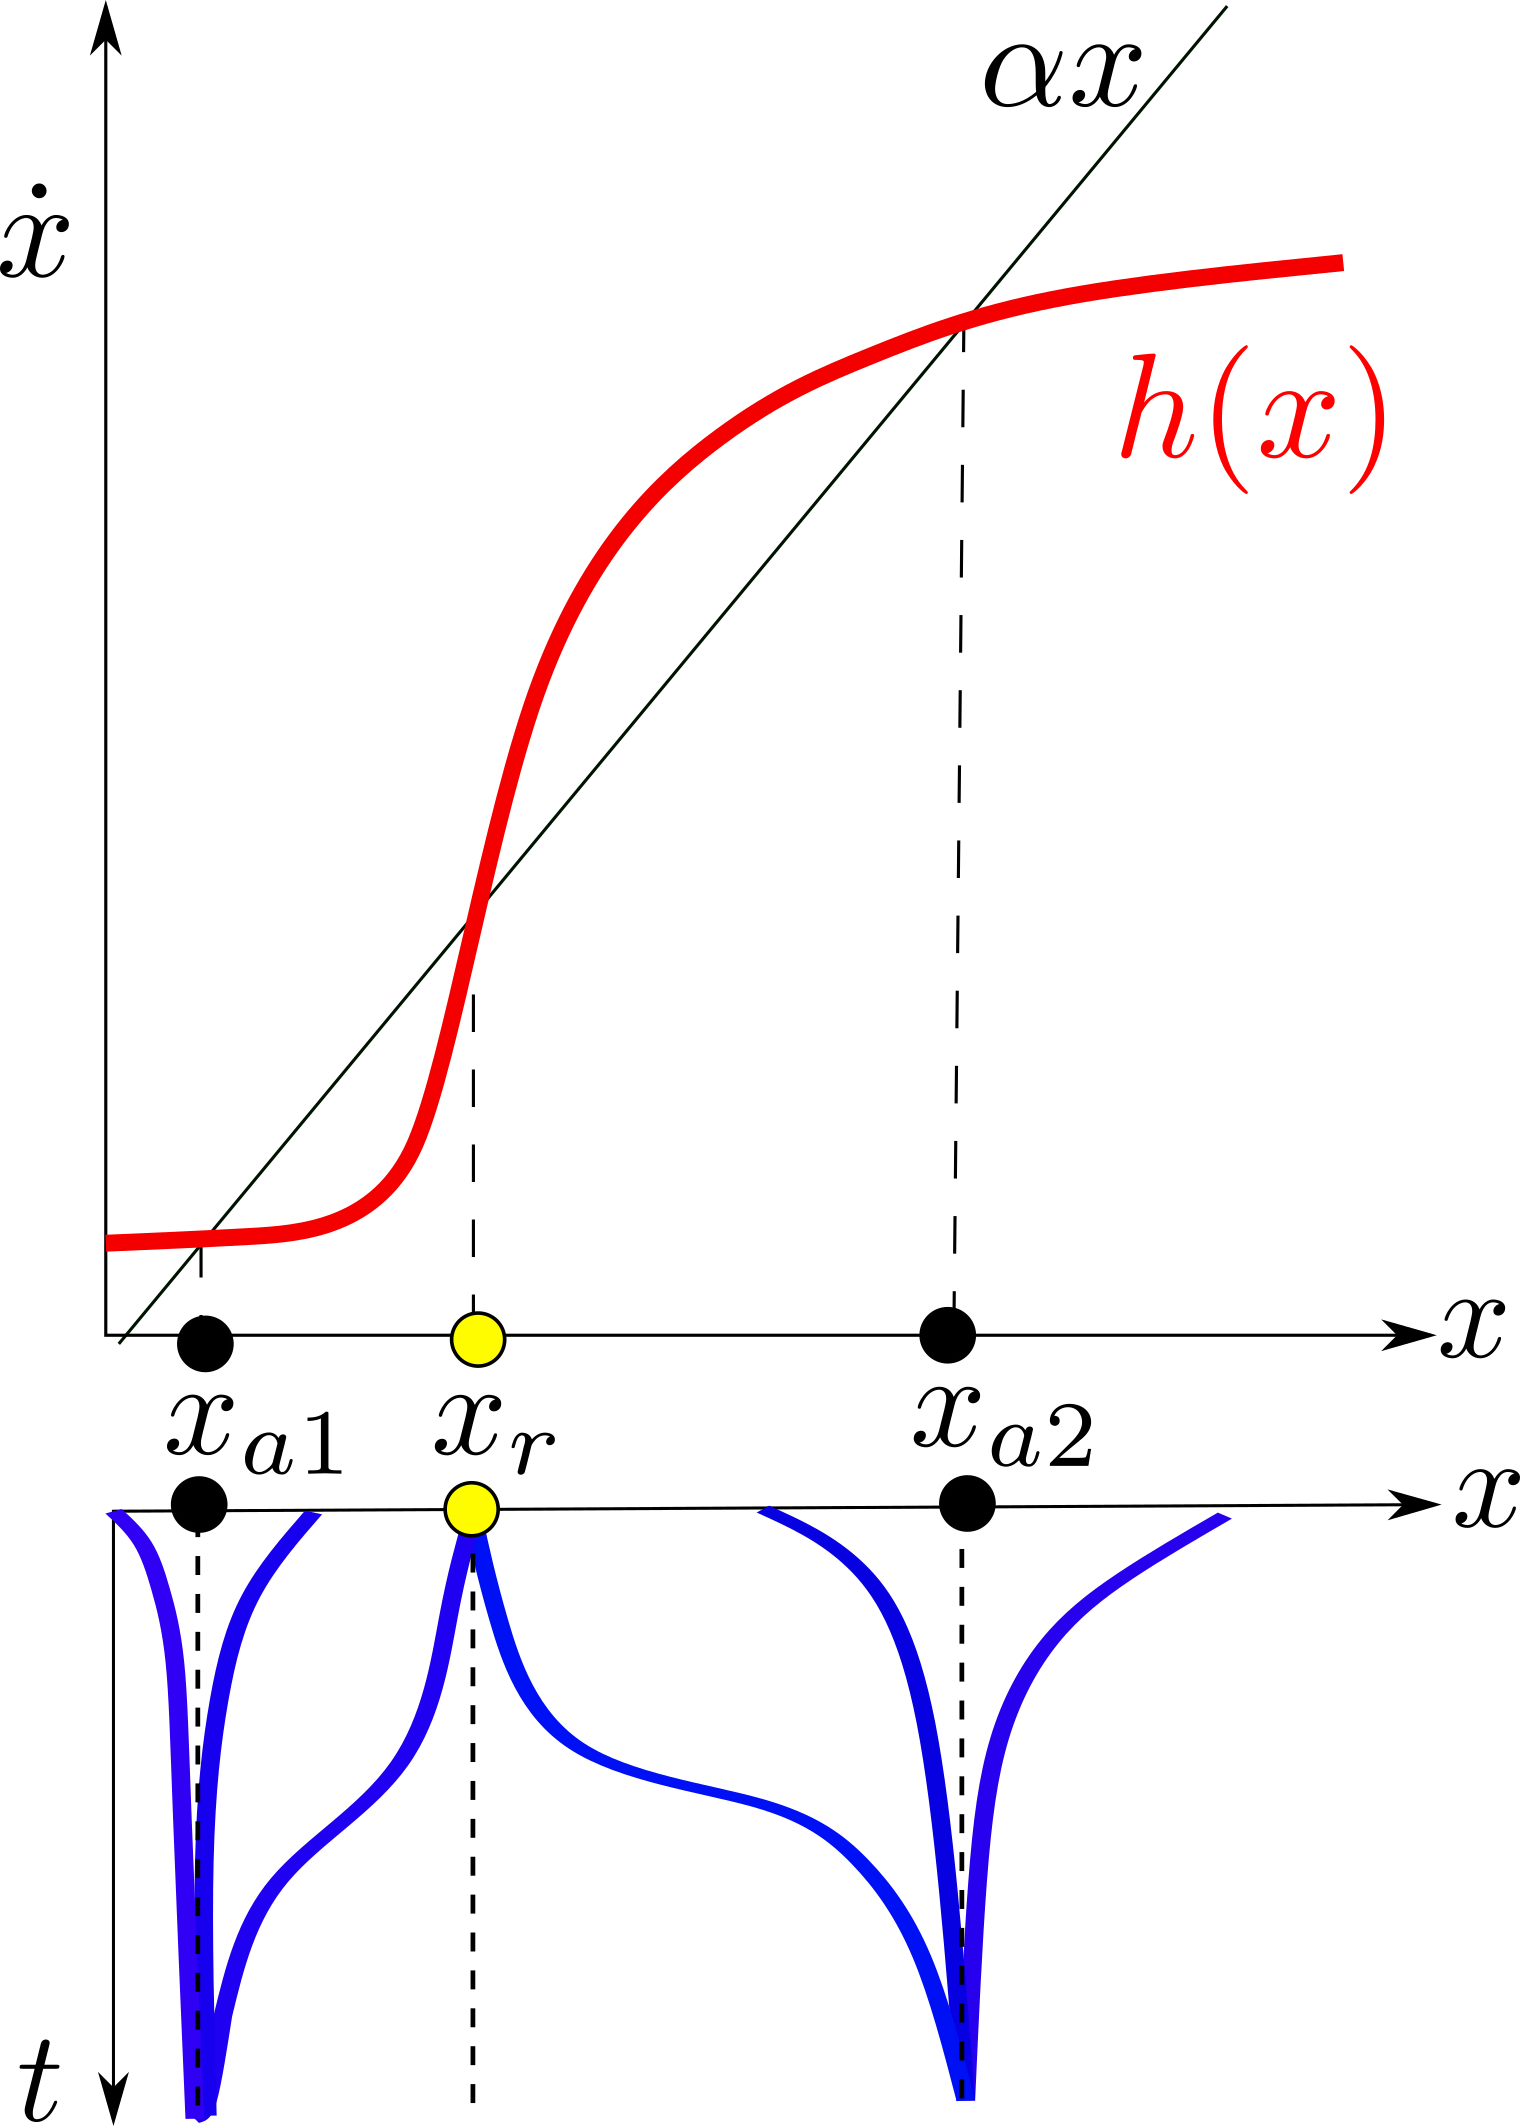
\includegraphics[width=2in]
{autoregulons/source-sink-source.png}
\caption{For single autoregulon $\dot{x}(t)=-\alp x + f(x)$, $(x, \dot{x})$ graphs and 
corresponding $(x,t)$ graphs. This $f()$ has
two repelling  points ($x_{r_1}, x_{r_2}$) 
and one attracting  point ($x_a$).
}
\label{fig-source-sink-source}
\end{figure}

\begin{figure}[h!]
\centering
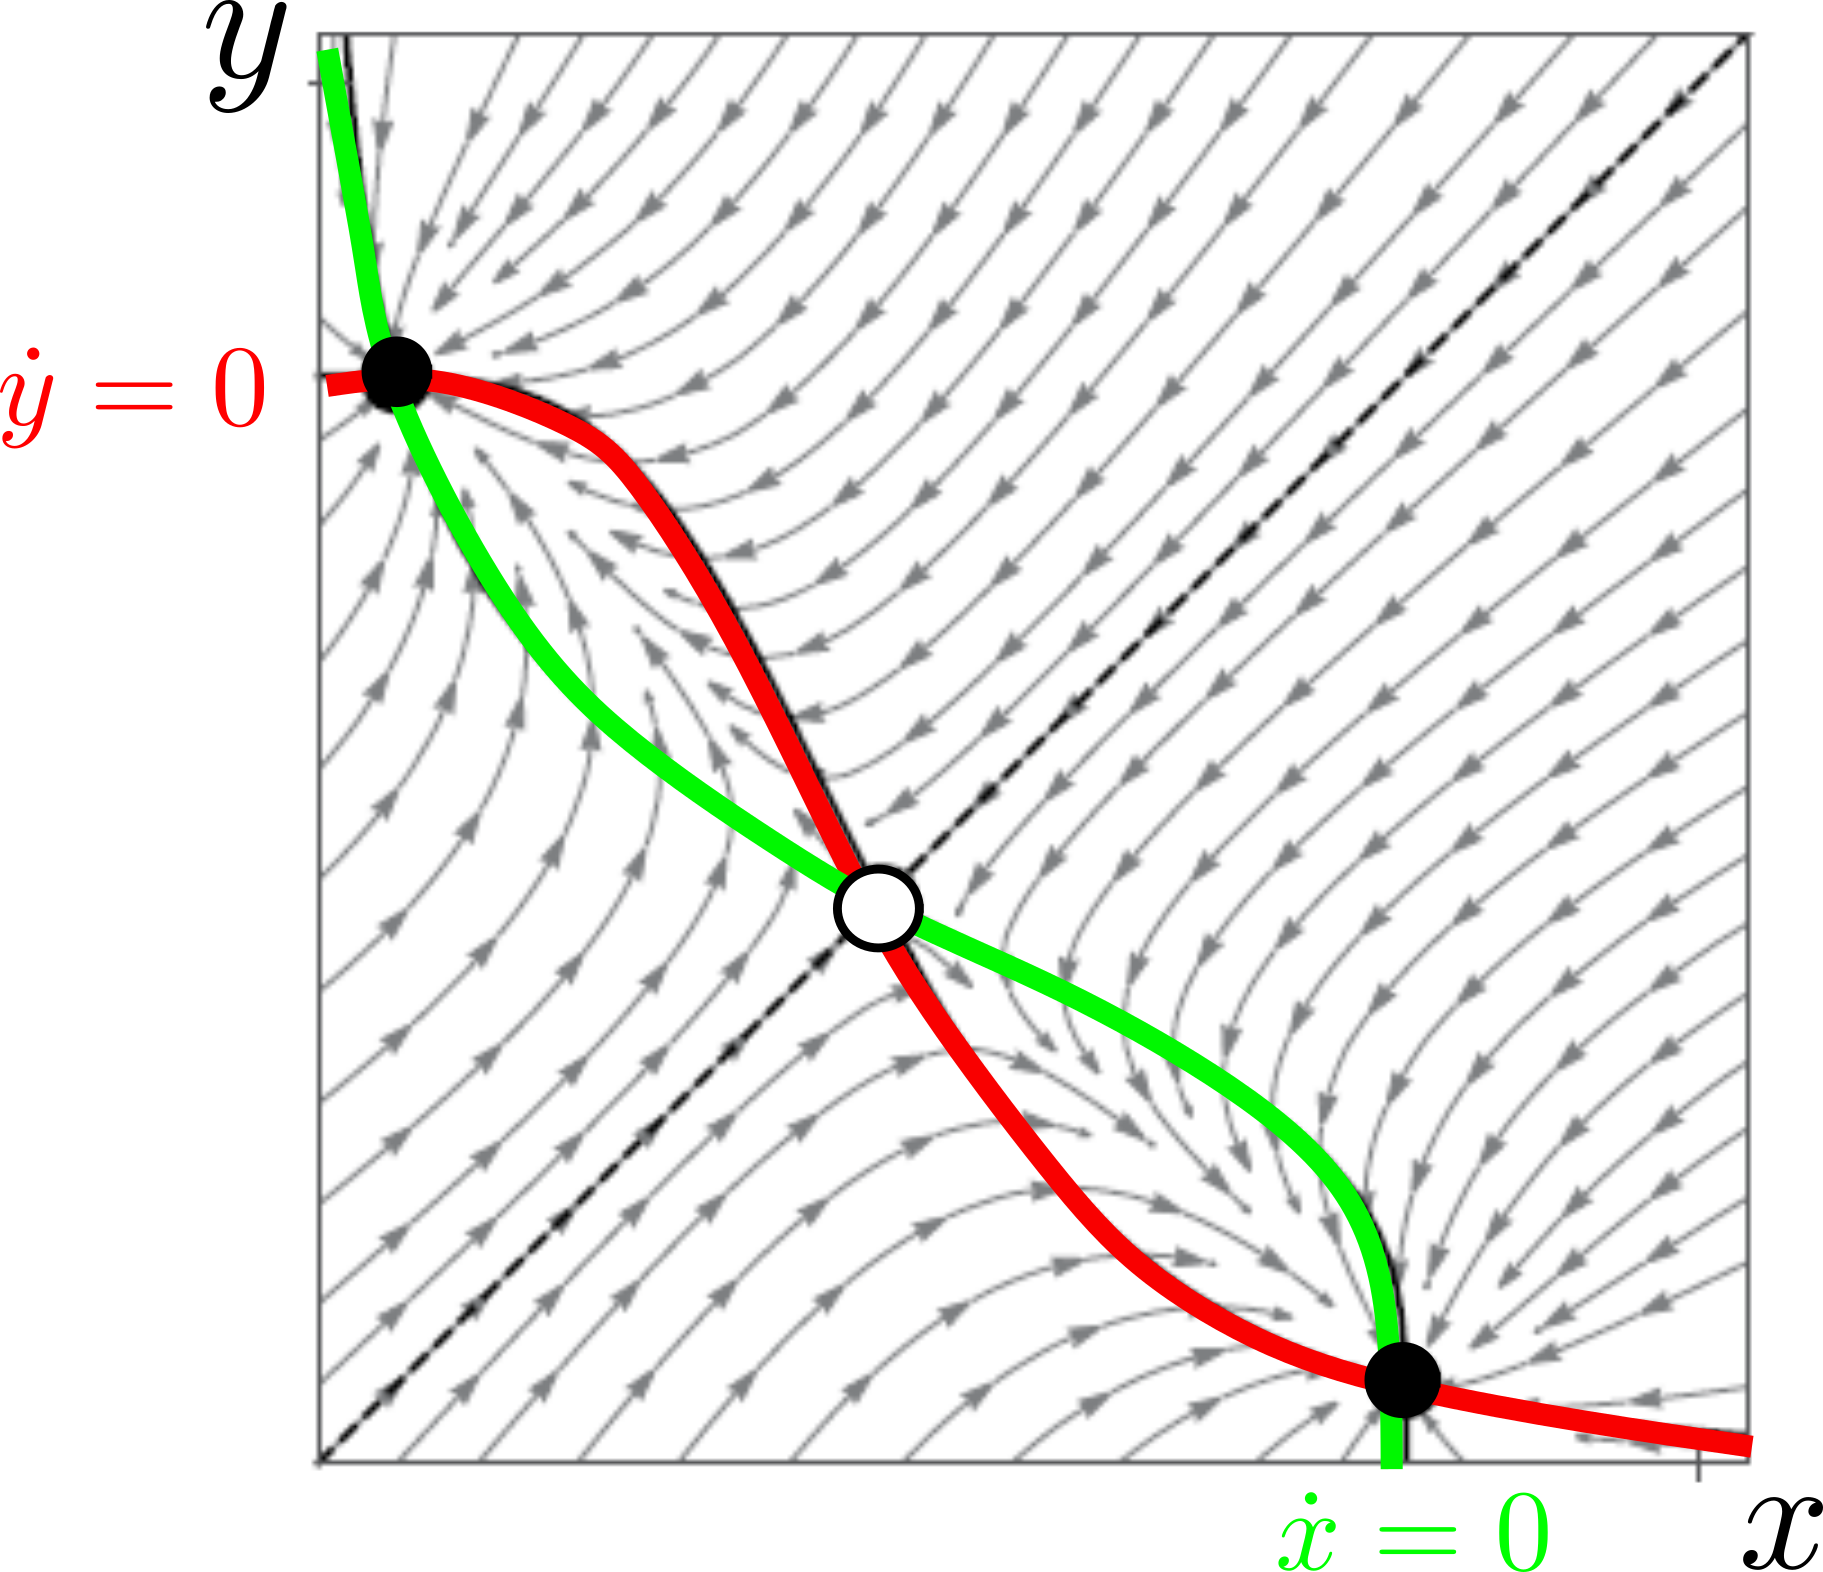
\includegraphics[width=3in]
{autoregulons/2dim-3fp.png}
\caption{Flow map for two autoregulons satisfyig Eqs.(\ref{eq-2dim-3fp}).}
\label{fig-2dim-3fp}
\end{figure}

\beq
\left\{
\begin{array}{l}
\dot{x} = -\alp y + f(x)
\\
\dot{y} =-\alp x + f(y)
\end{array}
\right.
\label{eq-2dim-3fp}
\eeq
Same $\alp$ and function $f()$ (shown in Fig.\ref{fig-source-sink-source}) for both differential
equations.


\section{Two autoregulons}

\begin{figure}[h!]
$$
\xymatrix@C=6pc@R=1pc{
\rvx \ar@{=>}[dd]\ar[ddr]|<<<<{}
& \rvy \ar@{=>}[dd]\ar[ddl]|<<<<{}
\\
&
\\
\dot{\rvx}
&\dot{\rvy}
}
\xymatrix{\\
\quad=\quad}
\xymatrix@C=5pc{
\\
\Rect{\rvx}
\autoar{r}
{}
{}
&
\Rect{\rvy}}
$$
\caption{Two autoregulons connected to each other.}
\label{fig-2-autoregulons}
\end{figure}

\beq
\left\{
\begin{array}{l}
\cald\rvx = f_\rvx(x) + \gamma_{\rvy\rarrow\rvx}\;y
\\
\cald\rvy = f_\rvy(y) +\gamma_{\rvx\rarrow\rvy}\;x
\end{array}
\right.
\eeq







\begin{figure}[h!]
$$
\xymatrix@C=6pc@R=2pc{
\rvx \ar@{=>}[dd]\ar[ddrr]|<<<<{}
\ar[r]
&\bigotimes\ar[ddl]\ar[ddr]
& \rvy \ar@{=>}[dd]\ar[ddll]|<<<<{}
\ar[l]
\\
&
\\
\dot{\rvx}
&
&\dot{\rvy}
}
\xymatrix{\\
\quad=\quad}
\xymatrix@C=5pc{
\\
\Rect{\rvx}
\wideautoar{r}
{}
{}
\timesar{r}
&
\Rect{\rvy}}
$$
\caption{Two autoregulons connected to each other, including population product (pp) term.}
\label{fig-2-autoregulons-pp}
\end{figure}

\beq
\left\{
\begin{array}{l}
\cald x = f_\rvx(\rvx) + g_\rvx(x, y)+ \gamma_{\rvy\rarrow\rvx}\;y
\\
\cald y = f_\rvy(\rvy) + g_\rvy(x, y) + \gamma_{\rvx\rarrow\rvy}\;x
\end{array}
\right.
\eeq

feedback

\subsection{Two Autoregulon Negative Feedback}

\begin{figure}[h!]
$$
\xymatrix@C=5pc
{\Rect{\rvx}
\autoar{r}{\redminus}{\redplus}
&\Rect{\rvy}
}
$$
\caption{Net for Two Autoregulon Negative Feedback (2AR-NF)}
\label{fig-2ar-nf}
\end{figure}

\subsection{Two autoregulon Positive Feedback}

\begin{figure}[h!]
$$
\xymatrix@C=5pc
{\Rect{\rvx}
\autoar{r}{\redminus}
{\redminus}
&\Rect{\rvy}
}\quad\quad
\xymatrix@C=5pc
{\Rect{\rvx}
\autoar{r}{\redplus}
{\redplus}
&\Rect{\rvy}
}
$$
\caption{Net for 2 Autoregulon Positive Feedback (2AR-PF)}
\label{fig-2ar-pf}
\end{figure}

\section{More than 2 autoregulons}

\begin{figure}[h!]
$$
\xymatrix@C=4pc@R=5pc{
&\Rect{\rvx}
\autoar{ld}{}{}
\autoar{rd}{}{}
\\
\Rect{\rvy}\autoar{rr}{}{}
&&
\Rect{\rvz}
}
$$
\caption{Three autoregulons connected to each other.
$\gamma_{\rvy\rarrow\rvx}$ coefficients are left implicit.}
\label{fig-3-autoregulons}
\end{figure}

\begin{figure}[h!]
$$
\begin{array}{ccc}
\xymatrix@C=4pc@R=5pc{
&\Rect{\rvx}
\autoar{ld}{-}{0}
\autoar{rd}{+}{0}
\\
\Rect{\rvy}\autoar{rr}{-}{0}
&&
\Rect{\rvz}
}
&&
\xymatrix@C=4pc@R=5pc{
&\Rect{\rvx}
\autoar{ld}{-}{0}
\autoar{rd}{+}{0}
\\
\Rect{\rvy}\autoar{rr}{+}{0}
&&
\Rect{\rvz}
}
\\
\\
(a)&&(b)
\end{array}
$$
\caption{$(a)$ shows a coherent net of 3 autoregulons because $\sign(\gamma_{\rvy\rarrow\rvz}\gamma_{\rvx\rarrow\rvy})=\sign(\gamma_{\rvx\rarrow\rvz})$.
$(b)$ shows a incoherent net of 3 autoregulons because $\sign(\gamma_{\rvy\rarrow\rvz}\gamma_{\rvx\rarrow\rvy})\neq \sign(\gamma_{\rvx\rarrow\rvz})$.
}
\label{fig-3-coherent-autoregulons}
\end{figure}




\beq
\left\{
\begin{array}{l}
\cald\rvx = f_\rvx(x)+
\gamma_{\rvy\rarrow\rvx}\;y
+
\gamma_{\rvz\rarrow\rvx}\;z
\\
\cald\rvy = f_\rvy(y)+
\gamma_{\rvx\rarrow\rvy}\;x
+
\gamma_{\rvz\rarrow\rvy}\;\rvz
\\
\cald\rvz = f_\rvz(z) +
\gamma_{\rvx\rarrow\rvz}\;x
+
\gamma_{\rvy\rarrow\rvz}\;y
\end{array}
\right.
\eeq

\begin{figure}
$$
\begin{array}{ccccc}
\xymatrix{
&\Rect{\rvx}\ar[dl]
\ar[dr]
\\
\Rect{\rvy}\ar[rr]
&&\Rect{\rvz}
}&
&
\xymatrix{
&\Rect{\rvx}\ar[dl]|\redoplus
\ar[dr]|\redoplus
\\
\Rect{\rvy}\ar[rr]|\redoplus
&&\Rect{\rvz}
}
&
&
\xymatrix{
&\Rect{\rvx}\ar[dl]|\redoplus
\ar[dr]|\redoplus
\\
\Rect{\rvy}\ar[rr]|\redominus
&&\Rect{\rvz}
}
\\
(a)
&&(b)
&&(c)
\end{array}
$$
\caption{$(a)$ Forward Feed Loop (FFL) net.
$(b)$ Coherent Type 1 FFL (C1-FFL).
$(c)$ Incoherent Type 1 FFL (I1-FFL)}

\end{figure}






%\begin{figure}[h!]
%$$
%\begin{array}{ccc}
%\xymatrix@C=3pc{
%&\Rect{\rvx}\ar[d]
%\ar[dl]|\redplus
%\\
%\Rect{\rvy}\ar[r]
%&
%\bigotimes\ar[r]|\redplus
%&\Rect{\rvz}
%}
%&
%&
%\xymatrix@C=3pc{
%&\Rect{\rvx}\ar[d]
%\ar[dl]|\redplus
%\\
%\Rect{\rvy}\ar[r]
%&\bigotimes\ar[r]|\redminus
%&\Rect{\rvz}
%}
%\\
%(a)
%&
%&(b)
%\end{array}
%$$
%\caption{
%$(a)$ C1-FFL with product node.
%$(b)$ I1-FFL with product node}
%\end{figure}




Feedforward Loop (FFL).

Coherent/Incoherent Type 1 FFL (C1-FFL/I1-FFL) if $K_{\rvy\rarrow\rvz}$ is highpass/lowpass.
where parameters (i.e., $\alp_\rvy, \alp_\rvz, \beta_\rvy, \beta_{\rvz}$) are positive.

\begin{figure}[h!]
$$
\begin{array}{ccc}
\xymatrix{
\rvx \ar@/_1pc/[drr]|\redoplus
\ar[r]|\redoplus
&\bigotimes\ar@/_3pc/[drr]|{\redplus}
& \rvy\ar[d]|{\redminus}\ar[l]|
\redoplus
&\rvz\ar[d]|{\redminus}
\\
&
& \dot{y}
&
\dot{z} 
}
&&
\xymatrix{
\rvx \ar@/_1pc/[drr]|\redoplus\ar[r]|\redoplus
&\bigotimes\ar@/_3pc/[drr]|{\redplus}
& \rvy\ar[d]|{\redminus}\ar[l]|
\redominus
&\rvz\ar[d]|{\redminus}
\\
&
& \dot{y}
&
\dot{z} 
}
\\
\\
(a)&&(b)
\end{array}
$$
\caption{$(a)$ C1-FFL bnet.
Note that $\rvy\rarrow \otimes$
is highpass filter.
$(b)$ I1-FFL bnet. Note that $\rvy\rarrow \otimes$
is lowpass filter.
}
\label{fig-bnet-c1-ffl}
\end{figure}


\beq
\left\{
\begin{array}{l}
\dot{y} =-\alp_\rvy y + \beta_\rvy \indi(x>K_{\rvx\rarrow\rvy}
)
\\
\dot{z} = -\alp_\rvz z + \beta_\rvz \indi(x> K_{\rvx\rarrow\rvz})
\left[
\begin{array}{ll}
\indi(y>K_{\rvy\rarrow\rvz})
&
\text{ if }
\rvy\rarrow\otimes\text{ is  highpass filter}
\\
\indi(y<K_{\rvy\rarrow\rvz})
&
\text{ if }
\rvy\rarrow\otimes\text{ is lowpass filter}
\end{array}
\right]
\end{array}
\right.
\label{eq-ffl-gen}
\eeq
where all the parameters (i.e., $\alp_\rvy, \alp_\rvz, \beta_\rvy, \beta_{\rvz}$) are positive.


\begin{figure}[h!]
\centering
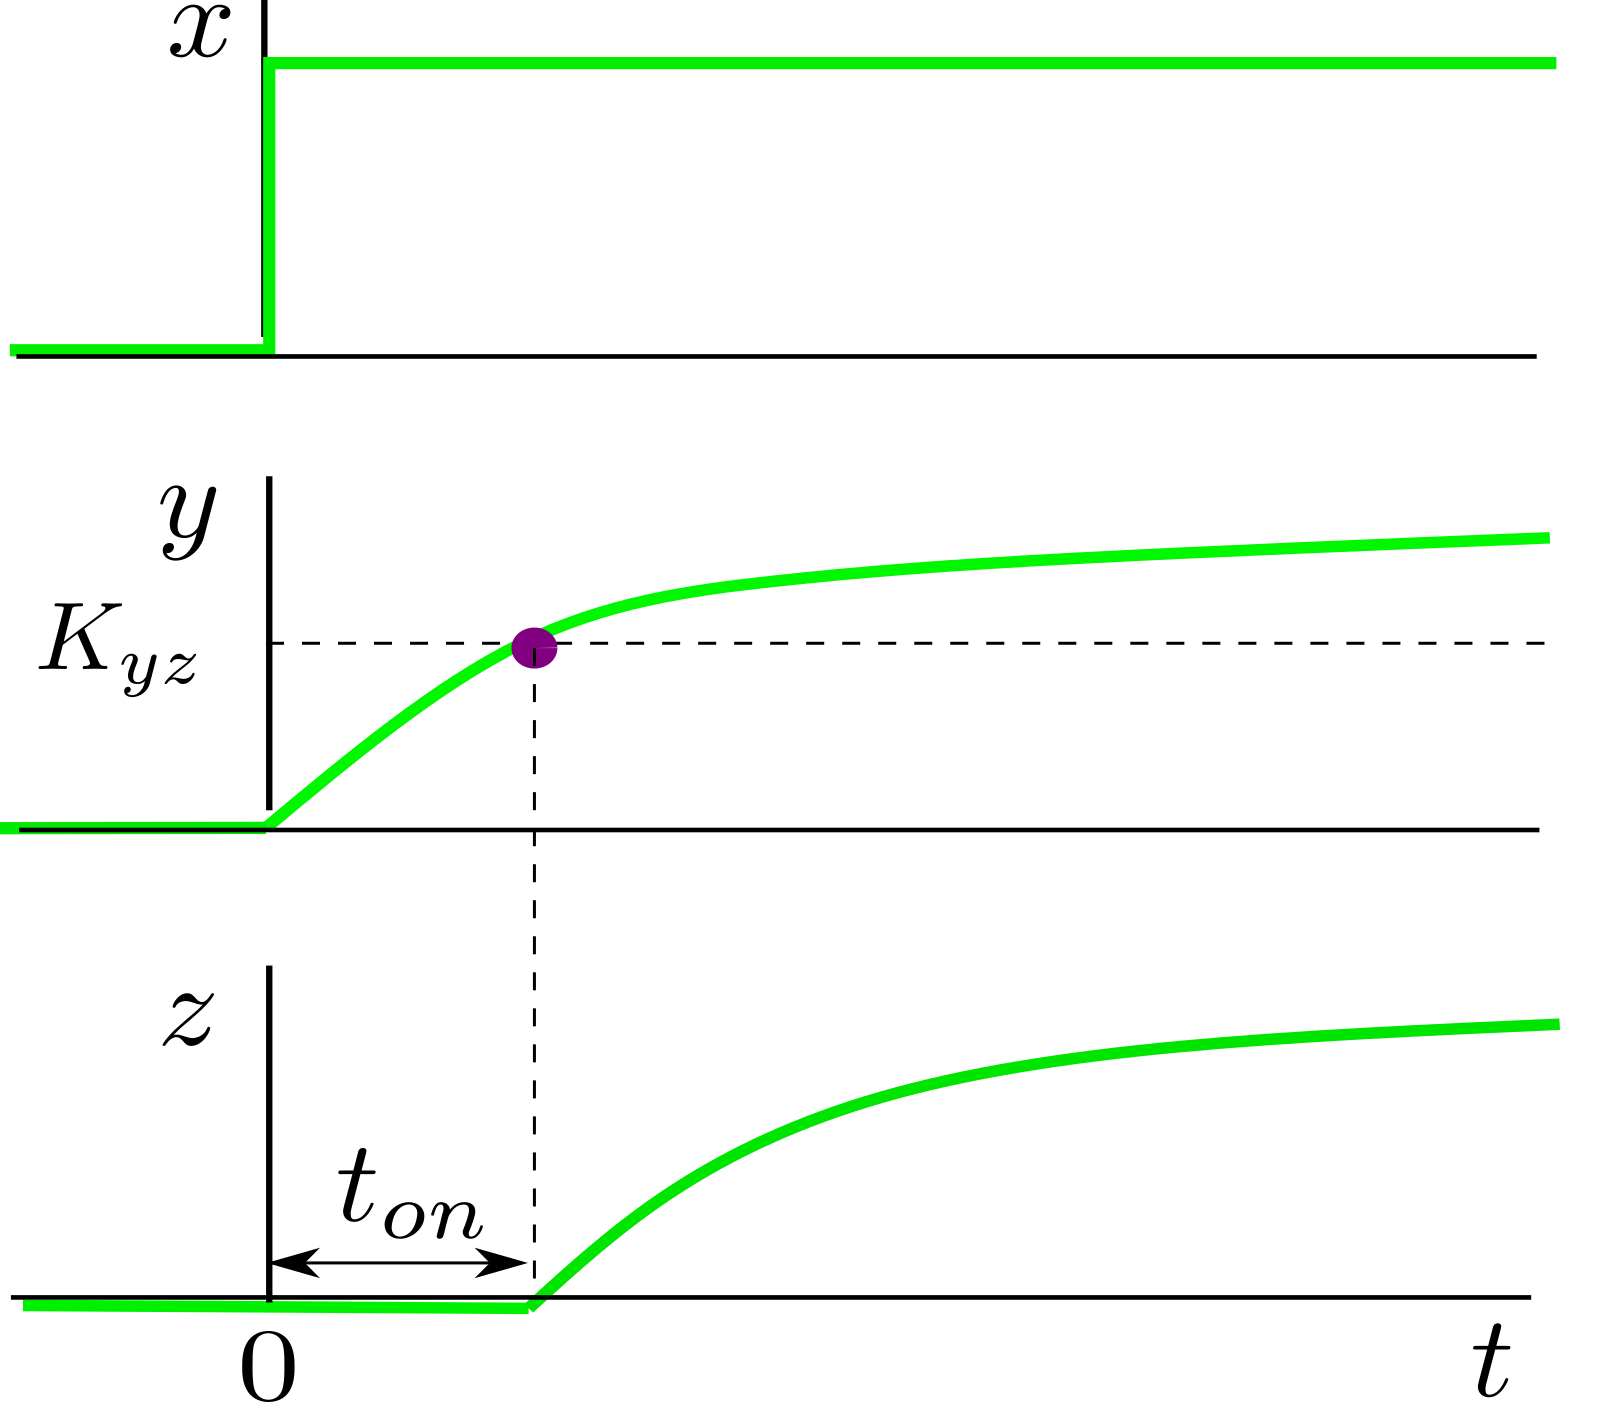
\includegraphics[height=2in]
{autoregulons/c1-ffl-up-green.png}
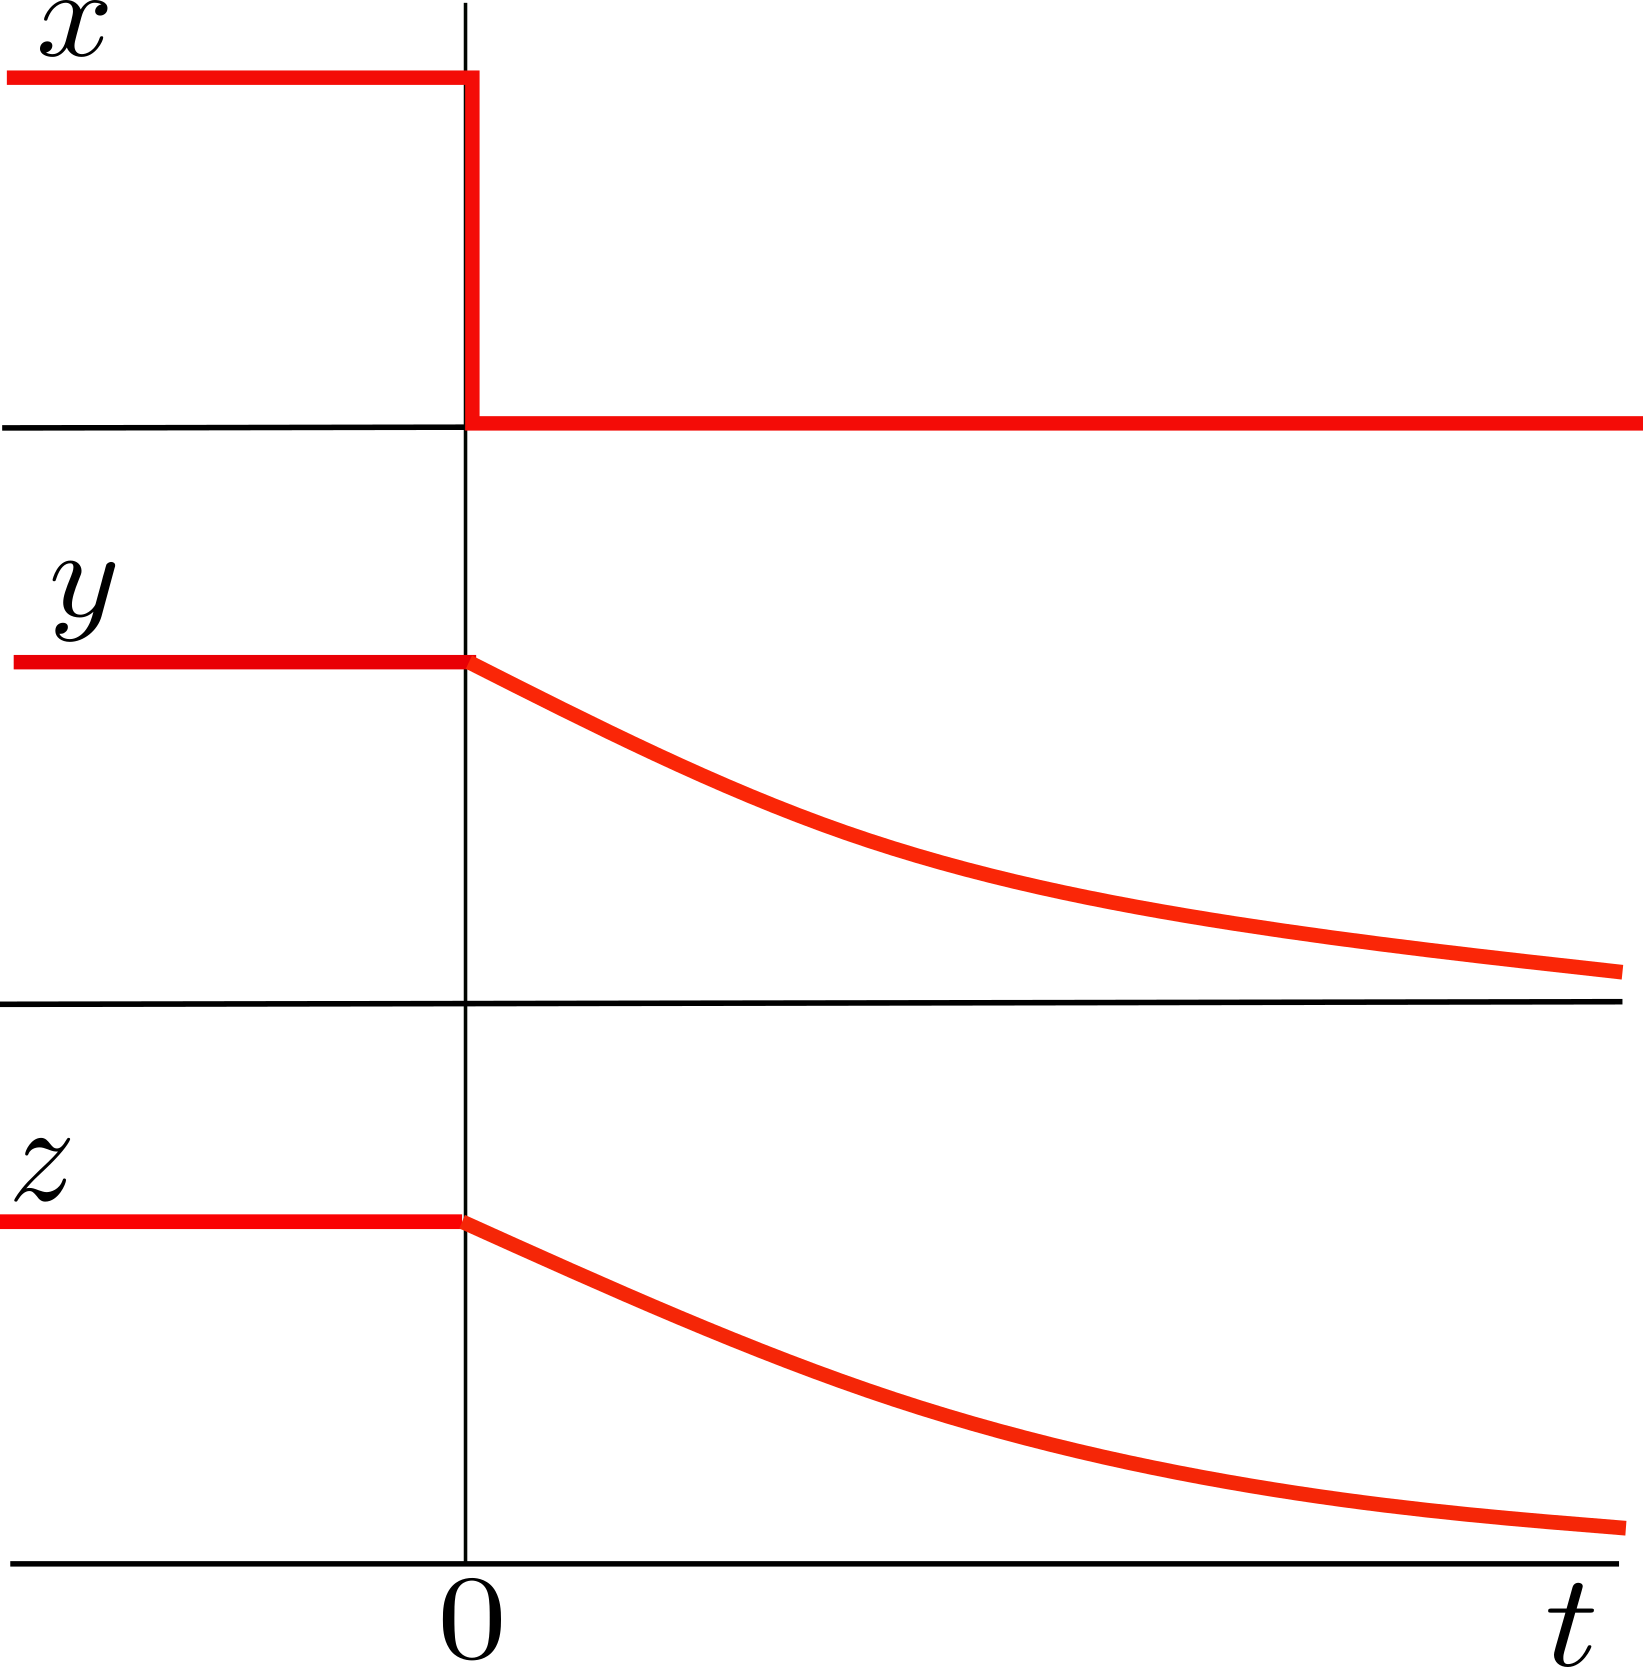
\includegraphics[height=2in]
{autoregulons/c1-ffl-down-green.png}
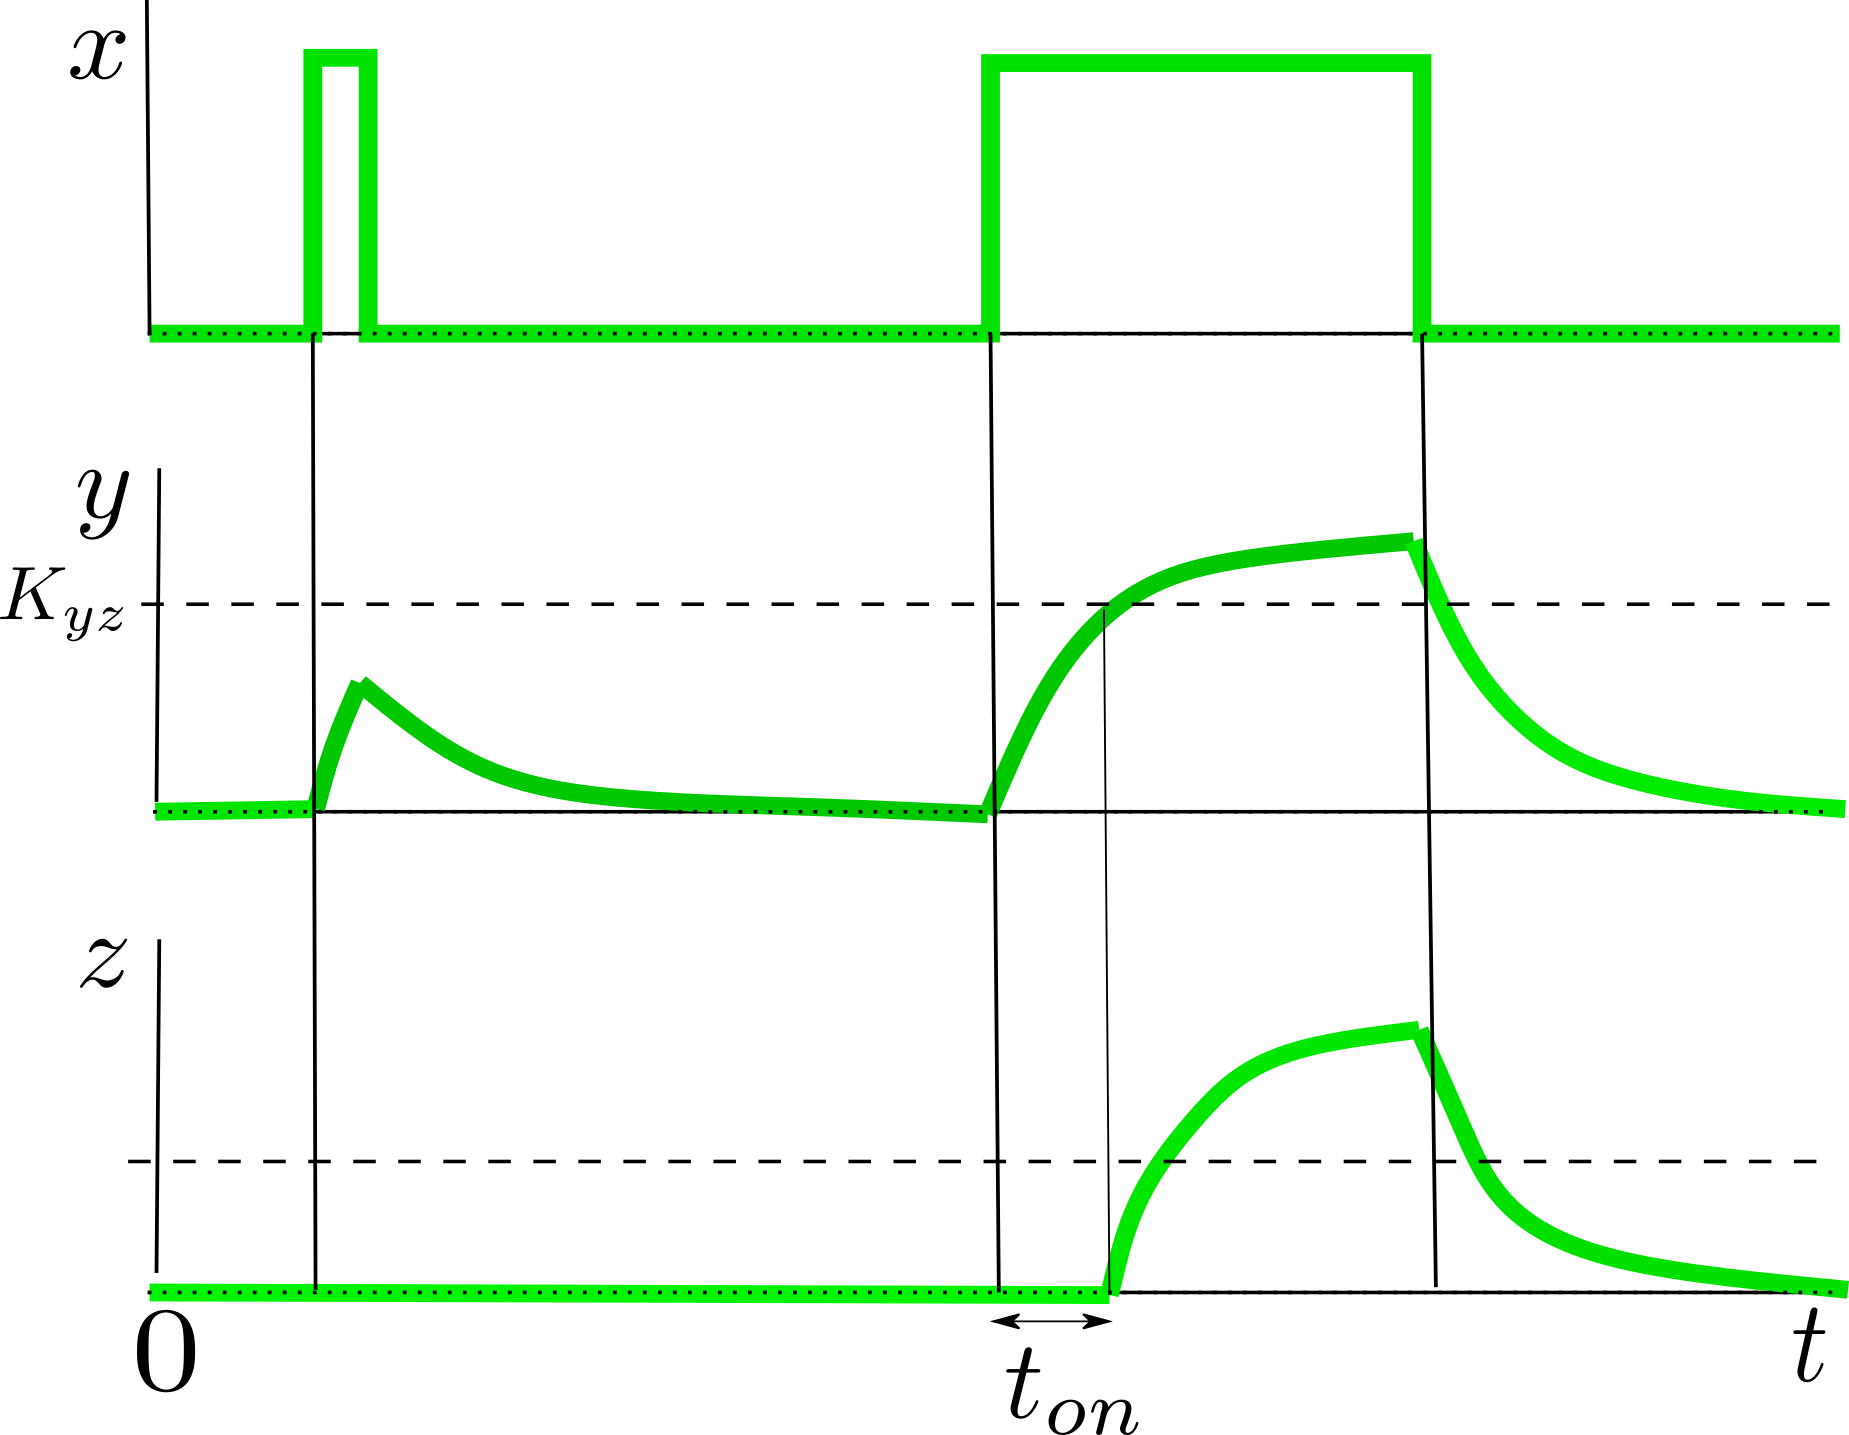
\includegraphics[height=2in]
{autoregulons/c1-ffl-up-down-green.png}
\caption{For C1-FFL, $x(t)$, $y(t)$, $z(t)$ assuming 
that $x(t)$ is either a rising step function (in green),
a dropping step function (in red),
or a square impulse function (in purple).}
\label{fig-c1-ffl-triple}
\end{figure}



\subsection{C1-FFL}
Below, the red equations 
correspond to a different choice of $x(t)$.

Assume (see Fig.\ref{fig-c1-ffl-triple})
\beq
x = x_0\indi(t>0)
\eeq
\beq \nonumber
\color{red}
x = x_0\indi(t<0)
\eeq
where $x_0 > K_{\rvx\rarrow\rvy}, K_{\rvx\rarrow\rvz}$.
Thus, Eq.(\ref{eq-ffl-gen}) reduces to

\beq
\left\{
\begin{array}{l}
\dot{y} = \beta_\rvy
-\alp_\rvy y
\\
\dot{z} =  \beta_\rvz
\indi(y>K_{\rvy\rarrow\rvz}) -\alp_\rvz z
\end{array}
\right.
\label{eq-ffl-red}
\eeq
Let $
y(0) = 0, y_{ss} = \frac{\beta_\rvy}{\alp_{\rvy}}
$.\
Then (see Fig.\ref{fig-c1-ffl-triple})

\beq
y = y_{ss}(1-e^{-\alp_\rvy t})
\eeq
\beq \nonumber \color{red}
y = y_0e^{-\alp_\rvy t}
\eeq
If $y_{ss}> K_{\rvy\rarrow\rvz}$
( or ${\color{red} y_0 < K_{\rvy\rarrow\rvz}}$), then (see Fig.\ref{fig-c1-ffl-triple})


\beq
z = \frac{\beta_\rvz}{\alp_\rvz}(1- e^{-\alp_\rvz (t-t_{on})})
\eeq
\beq\nonumber
\color{red}
z = z_0 e^{-\alp_\rvz t}
\eeq
where $t_{on}$ is defined so that

\beq
y(t_{on}) = K_{\rvy\rarrow\rvz}= y_{ss}(1-e^{-\alp_\rvy t})
\eeq
Solving the last equation for $t_{on}$ yields (see 
Fig.\ref{fig-minus-log-1-minus-x.png})

\beq
y_{on} = -\;\frac{1}{\alp_\rvy}
\ln
\left({1- \frac{K_{\rvy\rarrow\rvz}}{y_{ss}}}
\right)
\eeq

\begin{figure}[h!]
\centering
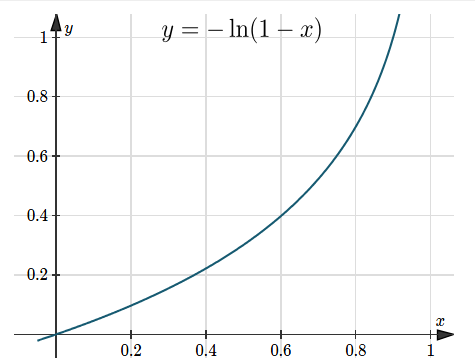
\includegraphics[width=2.8in]
{autoregulons/-log(1-x).png}
\caption{Plot of $y=-\ln(1-x)$.}
\label{fig-minus-log-1-minus-x.png}
\end{figure}

Fig.\ref{fig-c1-ffl-triple}
shows the waveforms for $x(t), y(t), z(t)$
assuming $x(t)$ is either 
a step function rising from 0 at $t=0$,
a step function falling to zero at $t=0$,
or a square impulse rising from 0 at time $t=0$
and falling to 0 a while later.

\subsection{I1-FFL}
\begin{figure}[h!]
\centering
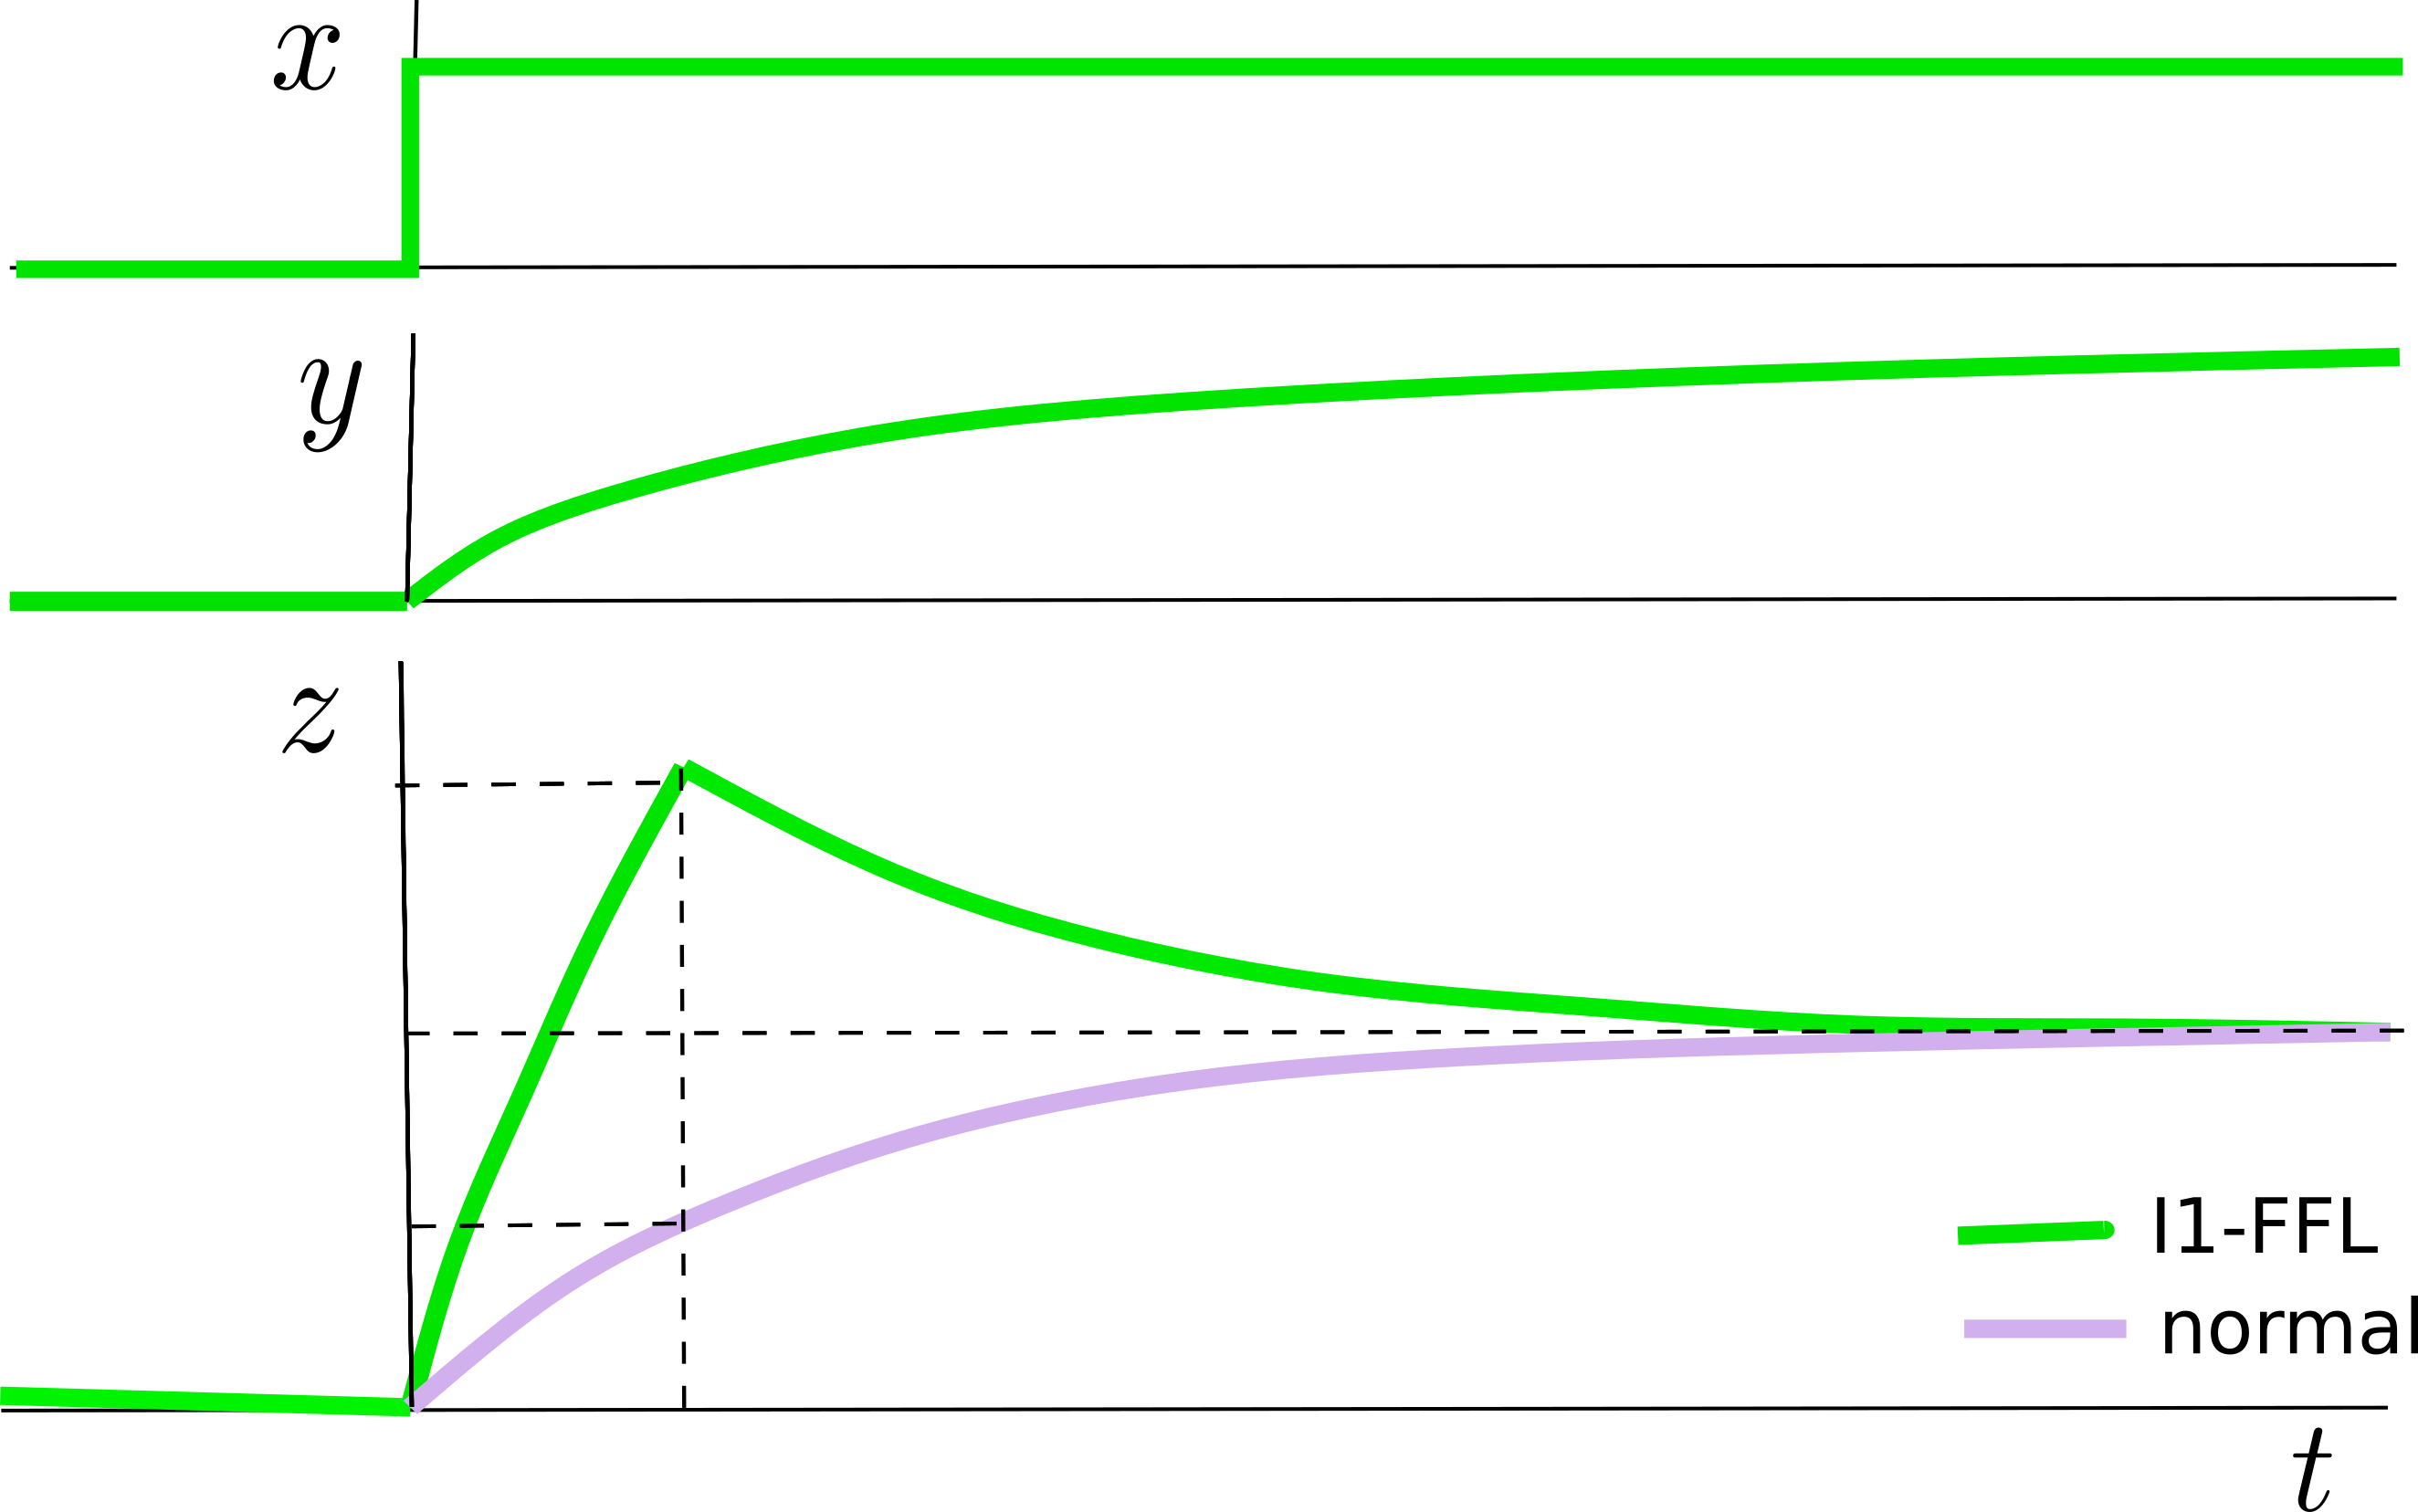
\includegraphics[width=2.8in]
{autoregulons/i1-ffl-green.png}
\caption{For I1-FFL, $x(t), y(t), z(t)$
assuming $x(t)$ step function rising 
from 0 at $t=0$.}
\label{fig-i1-ffl}
\end{figure}

\beq
z=\left\{
\begin{array}{ll}
\frac{\beta_z}{\alp_\rvz}(1- e^{-\alp_\rvz t})
& \text{ for } t<t_{max}
\\
y_{max}e^{-\alp_\rvz (t-t_{max})}
& \text{ for } t> t_{max}
\end{array}
\right.
\eeq
where 

\beq
y_{max}= \frac{\beta_\rvz}{\alp_\rvz}
(1-e^{-\alp_\rvz t_{max}})
\eeq

\subsection{Cascades of multiple autoregulons}

\begin{figure}[h!]
$$\begin{array}{ccc}
\xymatrix@C =3.5pc{
\Rect{\rvx}\ar[r]|\redplus
&\Rect{\rvy}\ar[r]|\redplus
&\Rect{\rvz}
}
&&
\xymatrix@C=3.5pc{
\Rect{\rvx}\ar[r]|\redminus
&\Rect{\rvy}\ar[r]|\redminus
&\Rect{\rvz}
}
\\
\\
(a)&&(b)
\end{array}
$$
\caption{Positive and Negative
cascades of autoregulons.}
\label{fig-cascade}
\end{figure}

\beq
\left\{
\begin{array}{l}
\dot{x}= -\alp_1 x
\\
\dot{y}= -\alp_2 y \pm \gamma_2 x
\\
\dot{z}= -\alp_3 z \pm \gamma_3 y
\end{array}
\right.
\eeq


\subsection{Repressilator}

\begin{figure}[h!]
$$
\xymatrix{
&\Rect{\rvx}\ar[dl]|\redminus
\\
\Rect{\rvy}\ar[rr]|\redminus
&&\Rect{\rvz}\ar[ul]|\redminus
}
$$
\caption{Repressilator net}
\label{fig-repress-net}
\end{figure}

\beq
\left\{
\begin{array}{l}
\dot{x}= -\alp_1 x - \gamma_1 z
\\
\dot{y}= -\alp_2 y - \gamma_2 x
\\
\dot{z}= -\alp_3 z - \gamma_3 y
\end{array}
\right.
\eeq

\subsection{Regulated feedback with 3 autoregulons}


\begin{figure}[h!]
$$
\xymatrix
{\Rect{\rvx}\ar[dr]
\autoar{rr}{}{}
&&\Rect{\rvy}\ar[dl]
\\
&\Rect{\rvz}
}
$$
\caption{Net for Regulated Feedback with 3 autoregulons. All 4 arrows can be either
$\redplus$ or $\redminus$.}
\label{fig-rf-3ar}
\end{figure}


\subsection{SIM net}
Single Input Module (SIM) net

\begin{figure}[h!]
$$
\xymatrix@R=4pc{
&\Rect{\rvx}
\ar[dl]|\redoplus_{K_1}
\ar[d]|\redoplus_{K_2}
\ar[dr]|\redoplus^{K_3}
\\
\Rect{\rvz_1}
&\Rect{\rvz_2}
&\Rect{\rvz_3}
}
$$
\caption{SIM net}
\label{fig-sim-gene-net}
\end{figure}


\beq
\left\{
\begin{array}{ll}
\dot{\rvx} =-\alp x +\beta\indi(x< K)
\\
\dot {\rvz_i} =-\alp x_i + \beta_i\indi(x>K_i)
& \text{for $i=1,2,3$}
\end{array}
\right.
\eeq

\begin{figure}[h!]
\centering
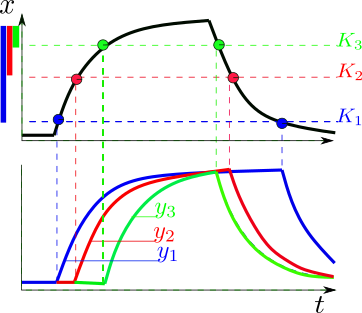
\includegraphics[width=2.8in]
{autoregulons/sim-net.png}
\caption{For SIM net, response  $z_1(t), z_2(t), z_3(t)$ to stimulus $x(t)$.}
\label{fig-sim-net}
\end{figure}


\newpage
\subsection{Flagellum net}

\begin{figure}[h!]
$$
\xymatrix@C=3pc{
&\Rect{\rvx}\ar[d]
\ar[ddl]|\redoplus_{K_1}
\ar[ddr]|\redoplus^{K_2}
\\
&\Rect{\rvy}\ar[dl]|\redoplus^{K'_1}
\ar[dr]|\redoplus_{K'_2}
\\
\Rect{\rvz_1}&
&\Rect{\rvz_2}
}
$$
\caption{Flagellum bnet. Assume $K_1<K_2$ and $K'_1 > K'_2$.}
\label{fig-flagellum}
\end{figure}

\begin{figure}[h!]
\centering
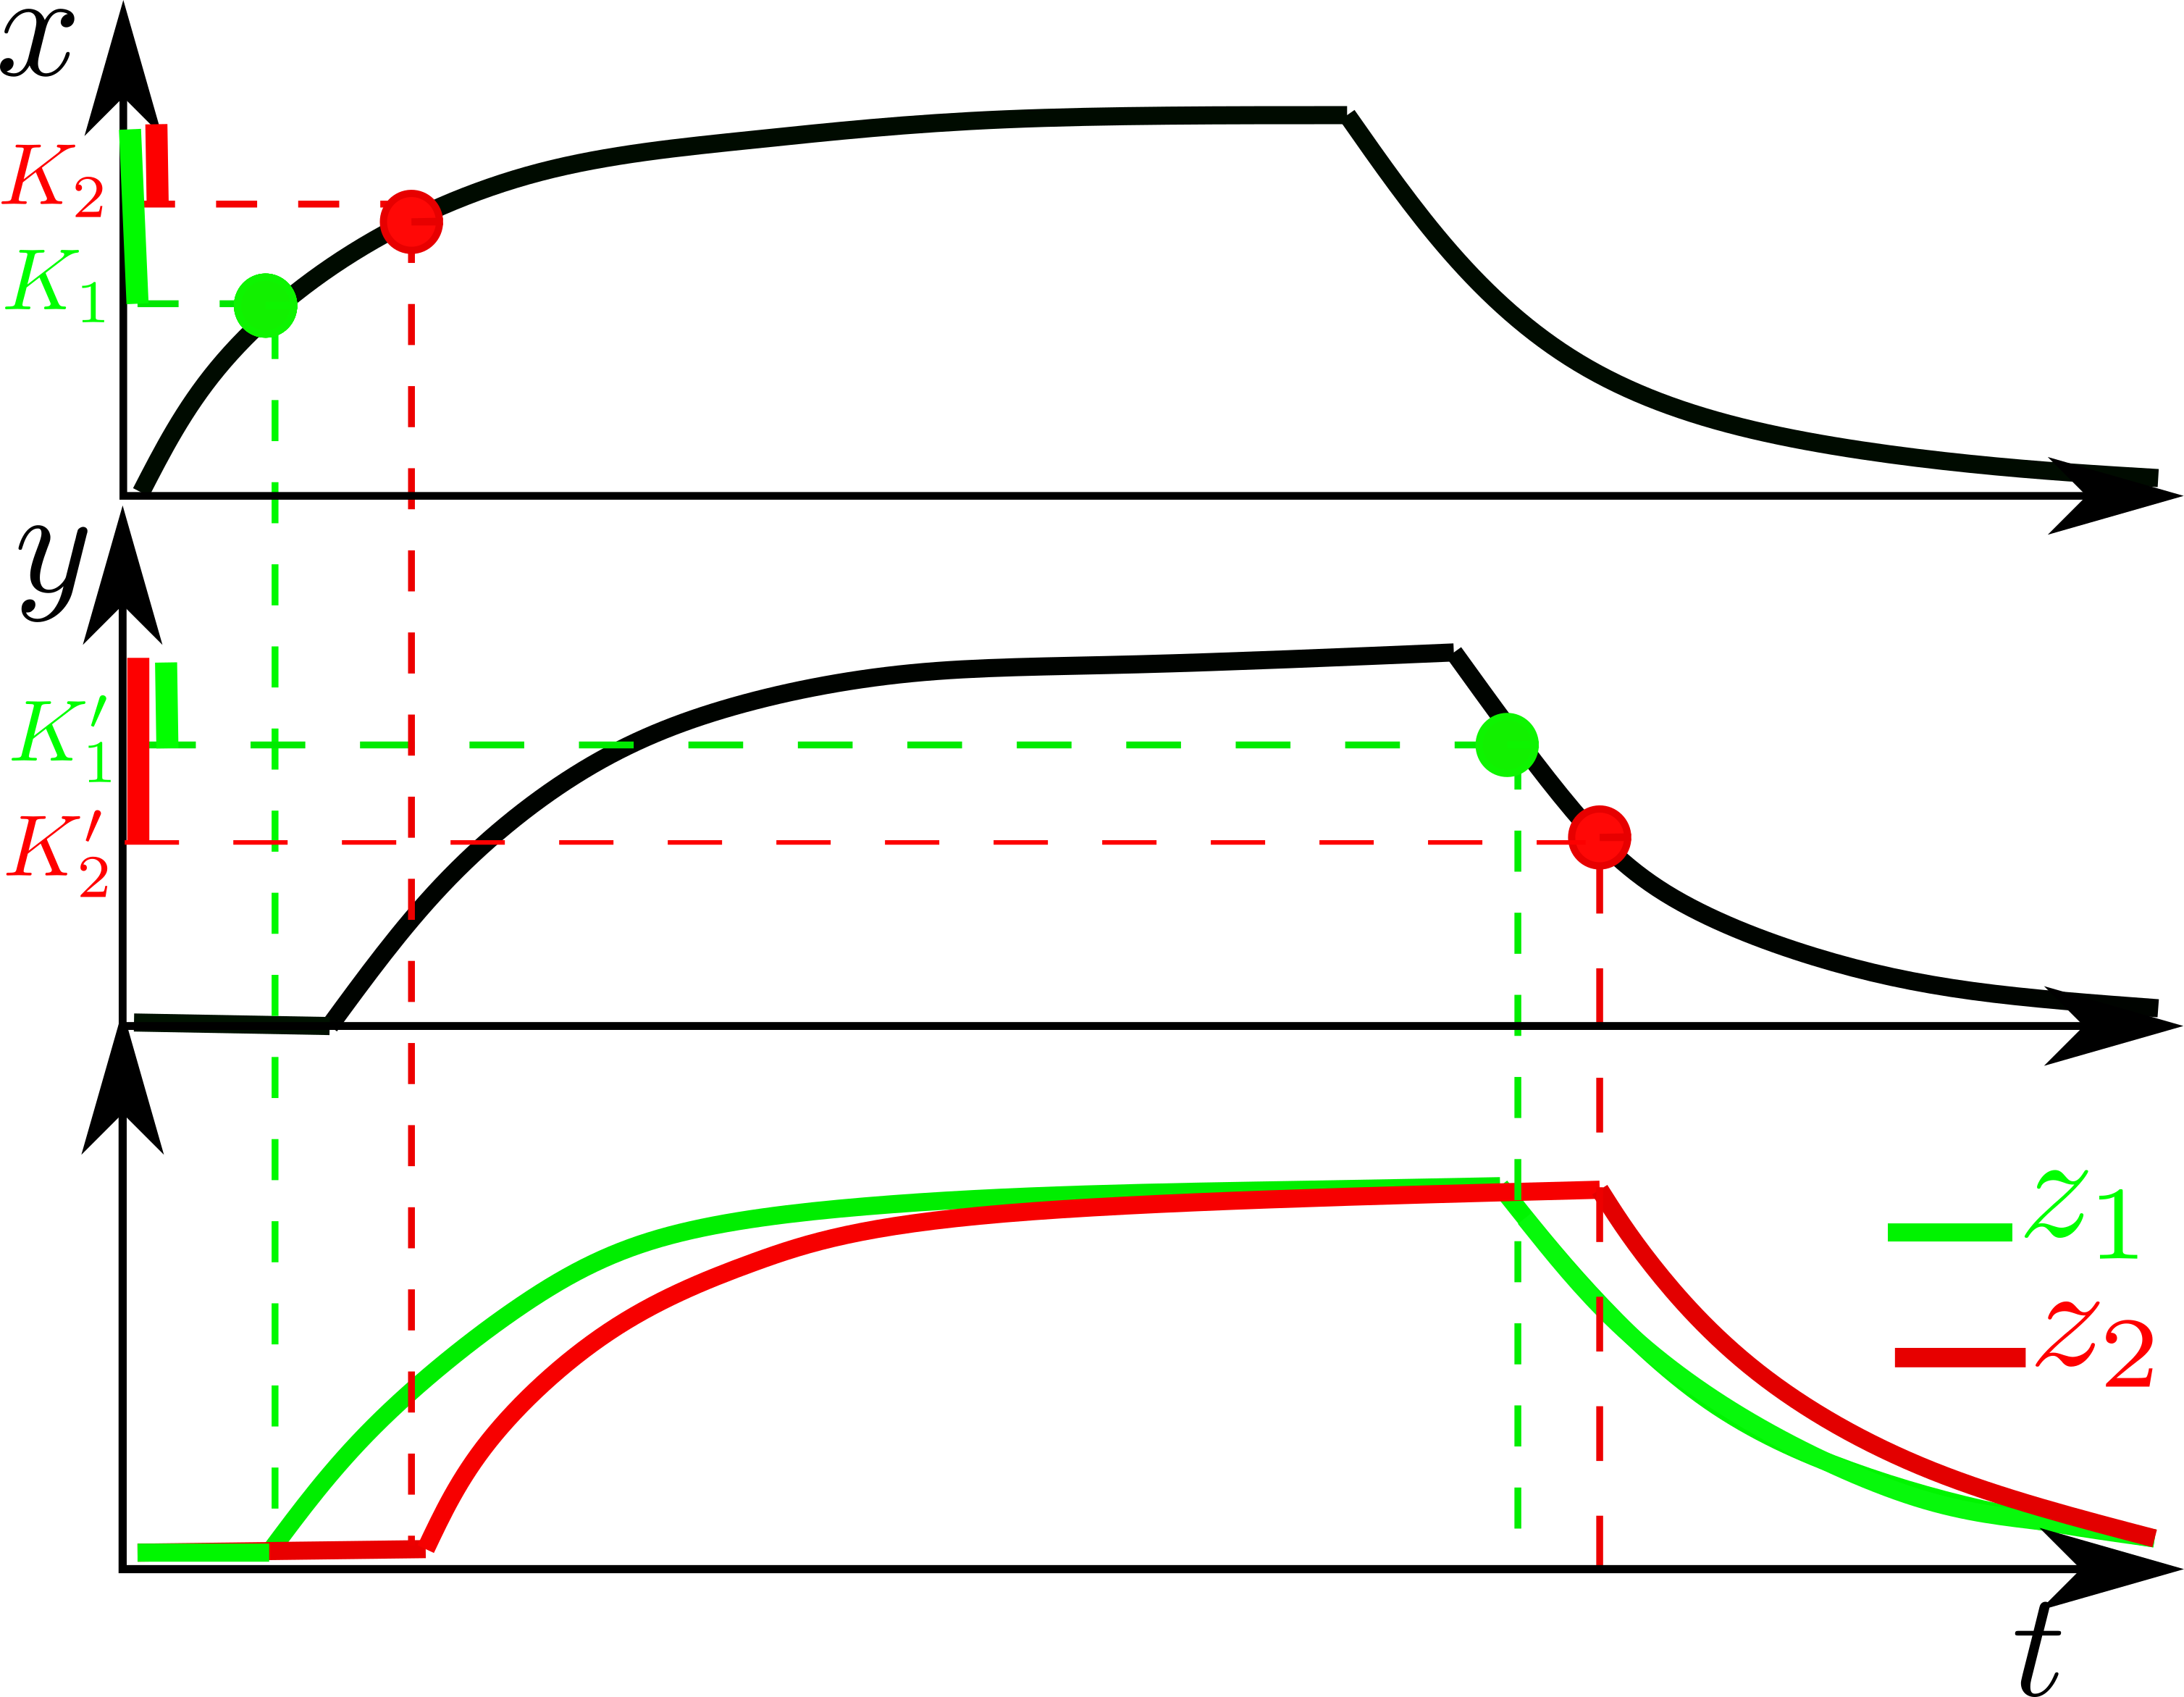
\includegraphics[width=2.8in]
{autoregulons/flagellum.png}
\caption{For Flagellum net, response  $y(t), z_1(t), z_2(t)$ to stimulus $x(t)$.}
\label{fig-flagellum-net}
\end{figure}


\subsection{Bacillus Subtilis Sporation net}

\begin{figure}[h!]
$$
\xymatrix{
&\Rect{\rvx_1}\ar[ddl]|\redplus
\ar[ddr]|\redplus
\\
&\Rect{\rvy_1}
\ar[dl]|\redminus
\ar[dr]|\redplus
\\
\bigotimes\ar[d]
&&\bigotimes\ar[d]
\\
\Rect{\rvz_1}
&&\Rect{\rvx_2}
\ar[d]|\redplus
\ar[ddl]|\redplus
\ar[ddr]|\redplus
\\
&&\Rect{\rvy_2}\ar[dl]|\redminus
\ar[dr]|\redplus
\\
&\bigotimes\ar[d]
&&\bigotimes\ar[d]
\\
&\Rect{\rvz_2}
&&\Rect{\rvz_3}
}$$
\caption{Bacillus Subtilis  Sporation net}
\label{fig-bac-sub}
\end{figure}


\subsection{Frog Egg Cell Cycle net}

\begin{figure}[h!]$$
\xymatrix@C=3pc
{\rvx_{u} \ar[rd]\ar@{=>}[d]\ar[r]
& \bigotimes\ar[dl]
& \rvx_p\ar[dr]
\ar[dl]|\redplus
\ar[l]|\redminus
\ar@{=>}[d]
& \rvy\ar[dl]\ar@{=>}[d]
\\
\dot{\rvx_{u}}
&\bigotimes\ar[r]
&\dot{\rvx_p}
&\dot{\rvy}}
$$
\caption{Frog egg cell cycle net}
\label{fig-frog-egg}
\end{figure}

\beq
\left\{
\begin{array}{l}
\dot{x_{u}}= -\calp x_{u} + \calp x_{u} - \calp x_{u}x_p
\\
\dot{x_p}= - \calp x_p  + \calp x_p +
\calp y+ \calp x_{u}x_p
\\
\dot{y}= -\calp y + \calp y + \calp x_p
\end{array}
\right.
\eeq

